\documentclass[12pt,t]{beamer}
\usepackage{hyperref}
\usepackage{localbeamer}
\usepackage{amsmath,amssymb}

\graphicspath{{./graphics/}}

\begin{document}

\title[Optimal Microfluidic Mixing and Cutoff]{Optimal Mixing in Microfluidic Channels\\ and the Cutoff Phenomenon}
\author{Matt West}
\institute[Stanford University]%
{Aeronautics and Astronautics, Stanford University\\
\url{http://www.stanford.edu/~westm/}}
\coauthor{Joint work with Tzu-Chen Liang}
\date{November 21, 2007}
\frame{\titlepage}

%%%%%%%%%%%%%%%%%%%%%%%%%%%%%%%%%%%%%%%%%%%%%%%%%%%%%%%%%%%%%%%%%%%%%%%
\begin{frame}
  \myframetitle{Microfluidic Mixing}
  \begin{itemize}
  \item Water in channel with cross-section $\ell \approx 100\,\mu\text{m}$.
  \item Reynold's number $\text{Re} = U\ell/\nu < 100$.
  \item P\'eclet number $\text{Pe} = U\ell/D \approx 10^6$.
  \item Required channel length $\gg 10\,\text{cm}$.
  \end{itemize}
  \begin{center}
      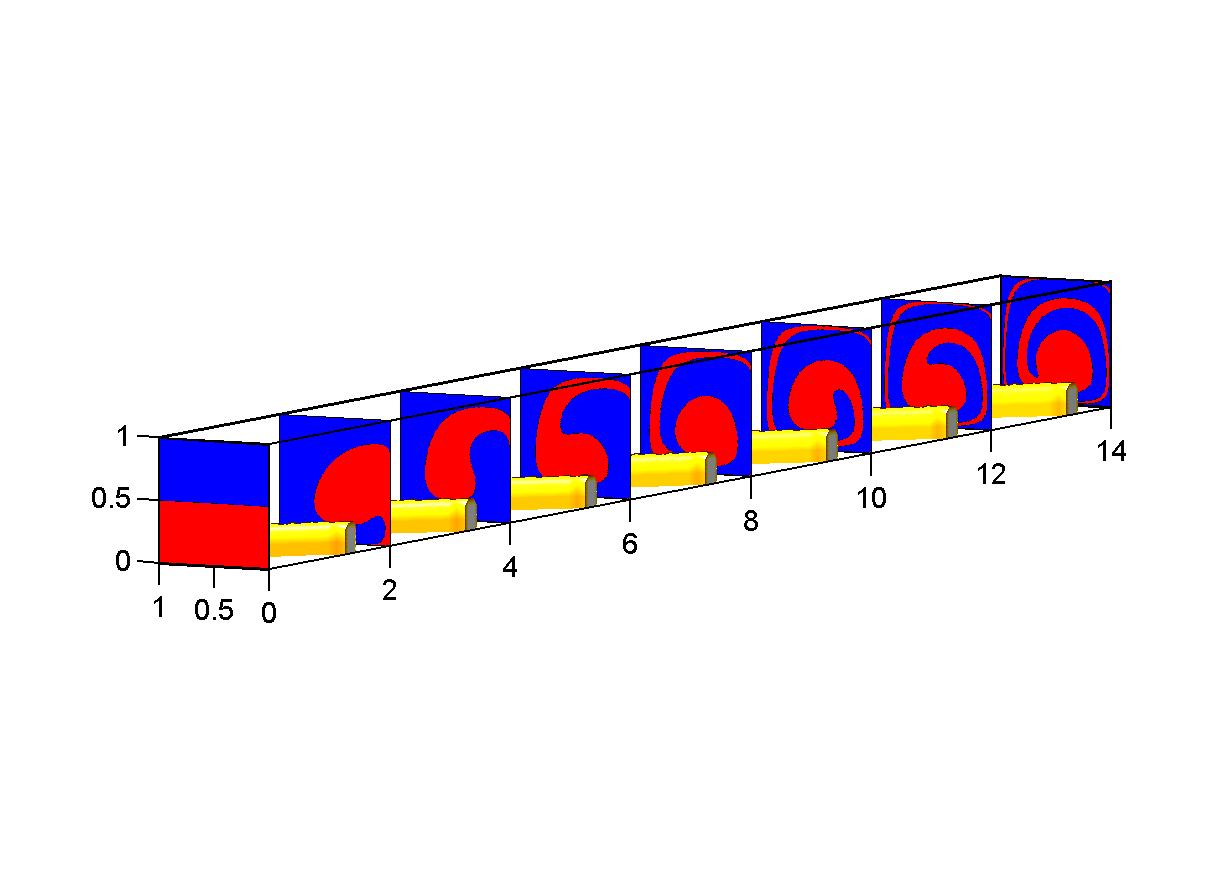
\includegraphics[height=4cm,trim=1.5cm 4cm 1.5cm 4.5cm,clip=true]{mixingchannel}
  \end{center}
\end{frame}
%%%%%%%%%%%%%%%%%%%%%%%%%%%%%%%%%%%%%%%%%%%%%%%%%%%%%%%%%%%%%%%%%%%%%%%
\begin{frame}
  \myframetitle{Staggered Herringbone Mixer}
  \begin{itemize}
  \item Stroock, Dertinger, Ajdari, Mezi\'c, Stone, Whitesides,
    \textit{Science} \textbf{295} (2002).
  \item Steady state flow produces chaotic map.
  \end{itemize}
  \begin{center}
    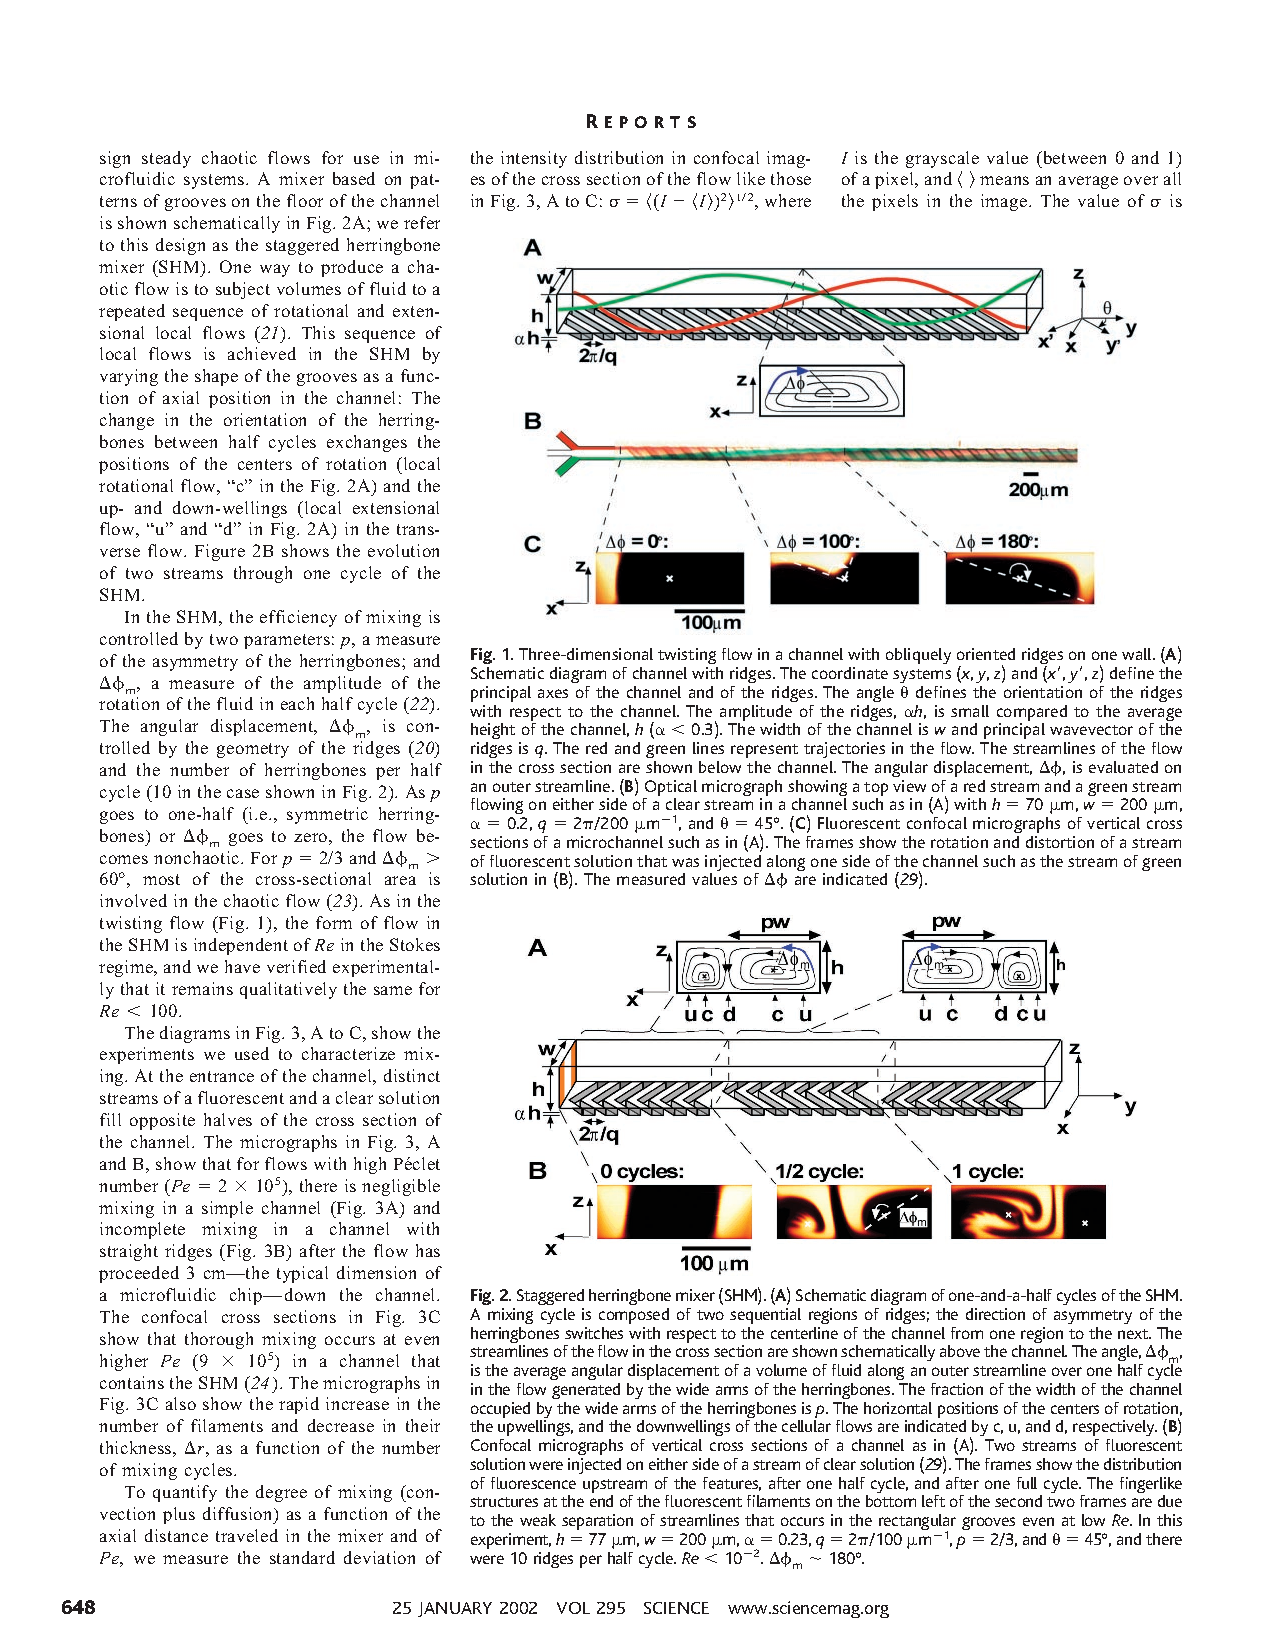
\includegraphics[height=5cm,trim=8.6cm 6.2cm 2cm 15.2cm,clip=true]{stroock_page2}
  \end{center}
\end{frame}
%%%%%%%%%%%%%%%%%%%%%%%%%%%%%%%%%%%%%%%%%%%%%%%%%%%%%%%%%%%%%%%%%%%%%%%
\begin{frame}
  \myframetitle{Mixing Measures}
  \begin{itemize}
  \item Specific initial condition (half colored).
  \item How mixed is a given state?
    \begin{itemize}
    \item $L_2$ with physical diffusion.
    \item $L_2$ of filtered state without diffusion.
    \item $H_{-1}$ without diffusion (also mix-norm of Mezi\'c).
    \end{itemize}
  \end{itemize}
  \begin{center}
    \hspace*{0.5cm}
    \hbox{\hbox{\vbox{\hbox{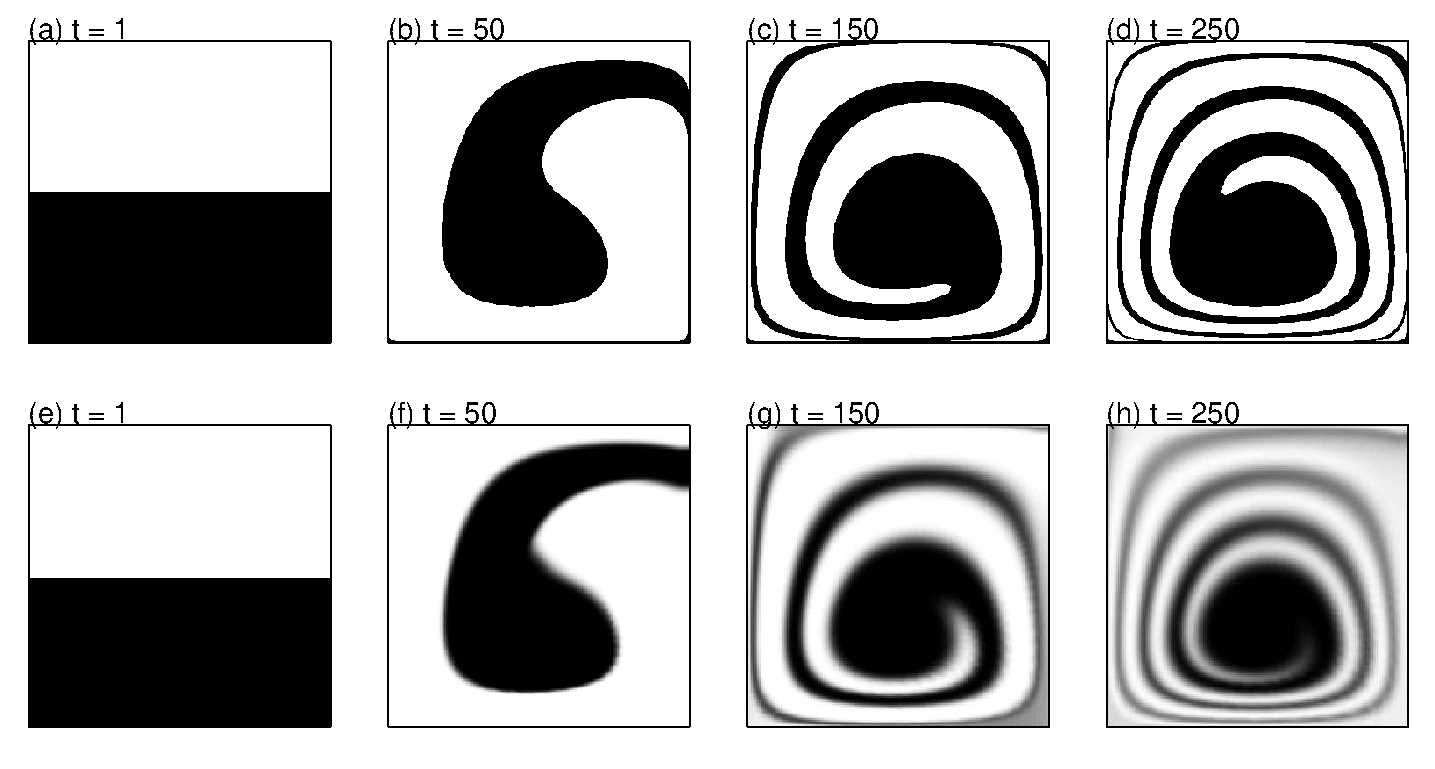
\includegraphics[width=5.5cm]{mixingcrosssectionreduced}}\hbox{\rule{0pt}{0.5cm}}}}
    \hbox{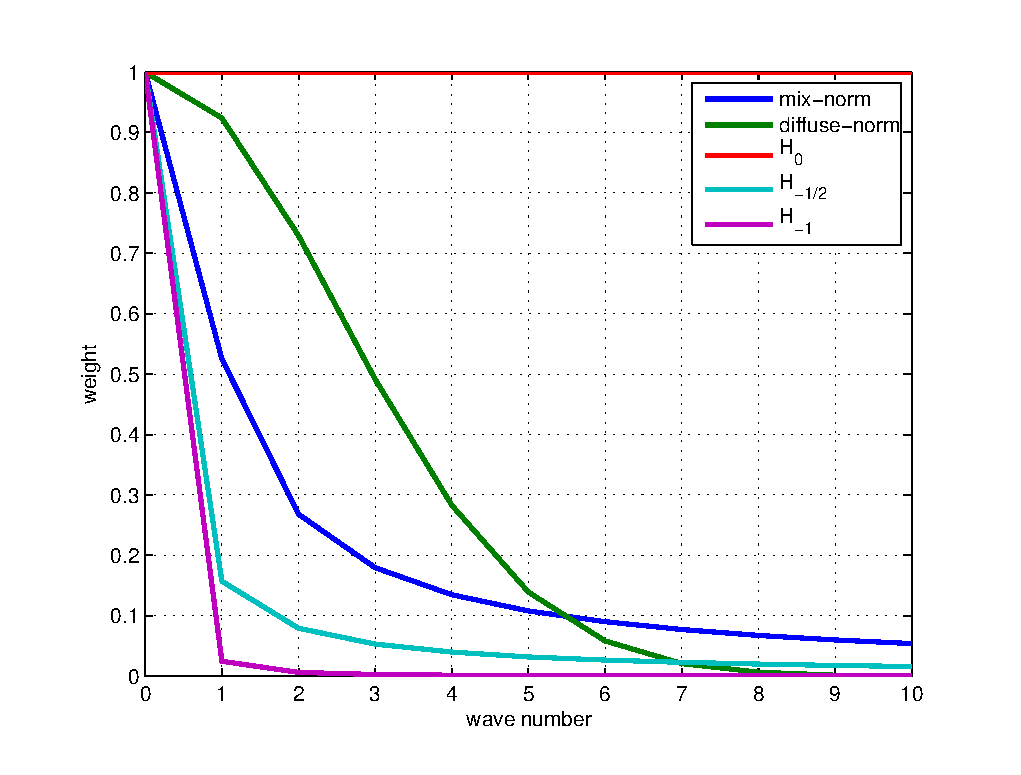
\includegraphics[width=5.5cm]{normcompare}}}
  \end{center}
\end{frame}
%%%%%%%%%%%%%%%%%%%%%%%%%%%%%%%%%%%%%%%%%%%%%%%%%%%%%%%%%%%%%%%%%%%%%%%
\begin{frame}
  \myframetitle{Transport Representations}
  \begin{itemize}
  \item Model as a stochastic map $[0,1]^2 \to [0,1]^2$.
  \item Approximate as a finite dimension Markov Chain on a regular
    grid (c.f. set-oriented numerics of Dellnitz)
    \begin{equation*}
      P_{ij} = \operatorname*{Prob}(x_{k+1} \text{ in cell } j \mid
      x_k \text{ in cell } i)
    \end{equation*}
  \item Perron-Frobenius operator maps probability distributions
    forward:
    \begin{equation*}
      \omega_{k+1} = P^T \omega
    \end{equation*}
  \item Koopman operator maps functions backwards:
    \begin{equation*}
      f_k = P f_{k+1}
    \end{equation*}
  \end{itemize}
\end{frame}
%%%%%%%%%%%%%%%%%%%%%%%%%%%%%%%%%%%%%%%%%%%%%%%%%%%%%%%%%%%%%%%%%%%%%%%
\begin{frame}
  \myframetitle{Topology Optimization}
  \begin{itemize}
  \item Model as Stokes flow in a complex geometry.
  \item Relaxation to porous structure $\longrightarrow$ Darcy flow.
    \begin{itemize}
    \item Velocity $u$, permeability $\alpha^{-1}$, pressure $p$,
      viscosity $\nu$, force $f$
    \end{itemize}
    \begin{align*}
      \label{stokes}
      (-\nu\Delta + \alpha) u +\nabla p &= f \\
      \operatorname*{div} u &= 0
    \end{align*}
  \item Gradient-based optimizers.
    \begin{itemize}
    \item We use steepest descent with line-search and inequality
      constraint projection.
    \end{itemize}
  \end{itemize}
\end{frame}
%%%%%%%%%%%%%%%%%%%%%%%%%%%%%%%%%%%%%%%%%%%%%%%%%%%%%%%%%%%%%%%%%%%%%%%
\begin{frame}
  \myframetitle{Objective Functions}
  \begin{itemize}
  \item Scalar cost function $g(u,p,\alpha)$
    \begin{align*}
      \text{minimize } & g(u,p,\alpha) \\
      \text{subject to } & \begin{bmatrix} -\nu L + \alpha H & G \\
        D & 0 \end{bmatrix} \begin{bmatrix} u \\ p \end{bmatrix}
      = \begin{bmatrix} f \\ 0 \end{bmatrix} \\
      & 0 \le \alpha \le \alpha_{\text{max}}
    \end{align*}
  \item Compute gradient with adjoint of constraint $R(u,p,\alpha) = 0$
    \begin{align*}
      \frac{d g}{d \alpha} &= \frac{\partial g}{\partial \alpha}
      + \frac{\partial g}{\partial u} \frac{\partial u}{\partial \alpha}
      &
      \frac{d R}{d \alpha} = \frac{\partial R}{\partial \alpha}
      + \frac{\partial R}{\partial u} \frac{\partial u}{\partial \alpha}
      &= 0 \\
      &= \frac{\partial g}{\partial \alpha}
      - \underbrace{\frac{\partial g}{\partial u}
      \left(\frac{\partial R}{\partial u}\right)^{-1}}_{x^T}
      \frac{\partial R}{\partial \alpha}
      &
      \left( \frac{\partial R}{\partial u} \right)^T x
      &= \left(\frac{\partial g}{\partial u} \right)^T
    \end{align*}
  \end{itemize}
\end{frame}
%%%%%%%%%%%%%%%%%%%%%%%%%%%%%%%%%%%%%%%%%%%%%%%%%%%%%%%%%%%%%%%%%%%%%%%
\begin{frame}
  \myframetitle{Objective Functions}
  \begin{itemize}
  \item Computationally cheap to use linear cost functions $g(u) = c^Tu$.
    \begin{itemize}
    \item As a heuristic we maximize downward velocity between the two
      vortices.
    \end{itemize}
  \item Alternative objective functions:
    \begin{itemize}
    \item Can differentiate particle streamlines with respect to $u$ and
      $\alpha$, allowing objective functions involving the particle map.
    \item Subgradients can be found for eigenvalues of the Markov
      matrix, allowing optimization of spectral mixing properties.
    \end{itemize}
  \item Compute with $144 \times 24 \times 72$ fluid/structure grid,
    $800 \times 1600$ color grid.
  \end{itemize}
\end{frame}
%%%%%%%%%%%%%%%%%%%%%%%%%%%%%%%%%%%%%%%%%%%%%%%%%%%%%%%%%%%%%%%%%%%%%%%
\begin{frame}
  \myframetitle{Optimal 3D Structure}
  \begin{itemize}
  \item Maximize downward velocity between vortices.
    \begin{itemize}
    \item Permeability relaxation vanishes at optimum.
    \end{itemize}
  \end{itemize}
  \begin{center}
    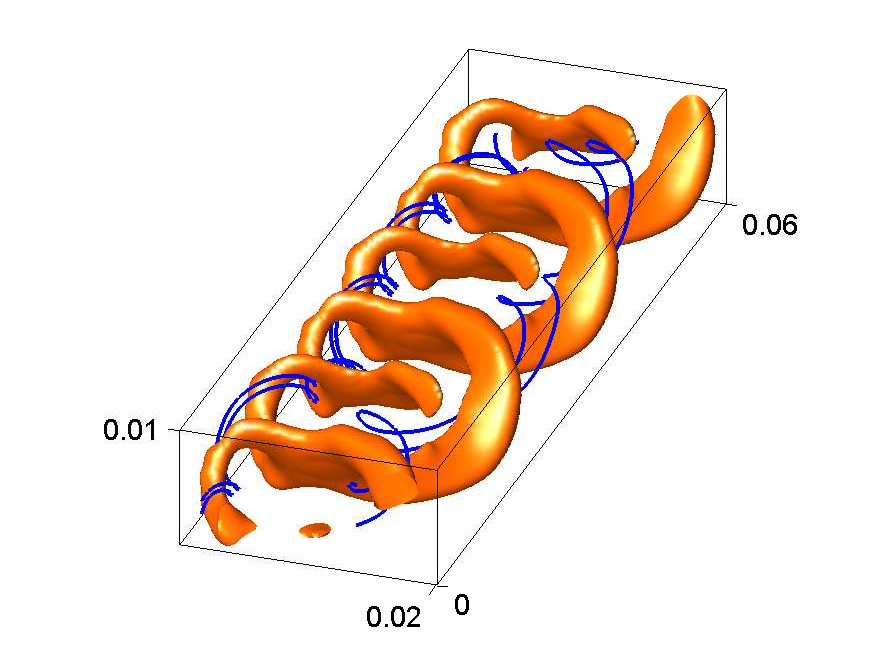
\includegraphics[height=6cm]{my3dstructure}
  \end{center}
\end{frame}
%%%%%%%%%%%%%%%%%%%%%%%%%%%%%%%%%%%%%%%%%%%%%%%%%%%%%%%%%%%%%%%%%%%%%%%
\begin{frame}
  \myframetitle{Optimal 2D Structure}
  \begin{itemize}
  \item Maximize downward velocity between vortices.
    \begin{itemize}
    \item Subject to $\alpha = 0$ away from channel edge (only surface
      structure).
    \end{itemize}
  \end{itemize}
  \begin{center}
    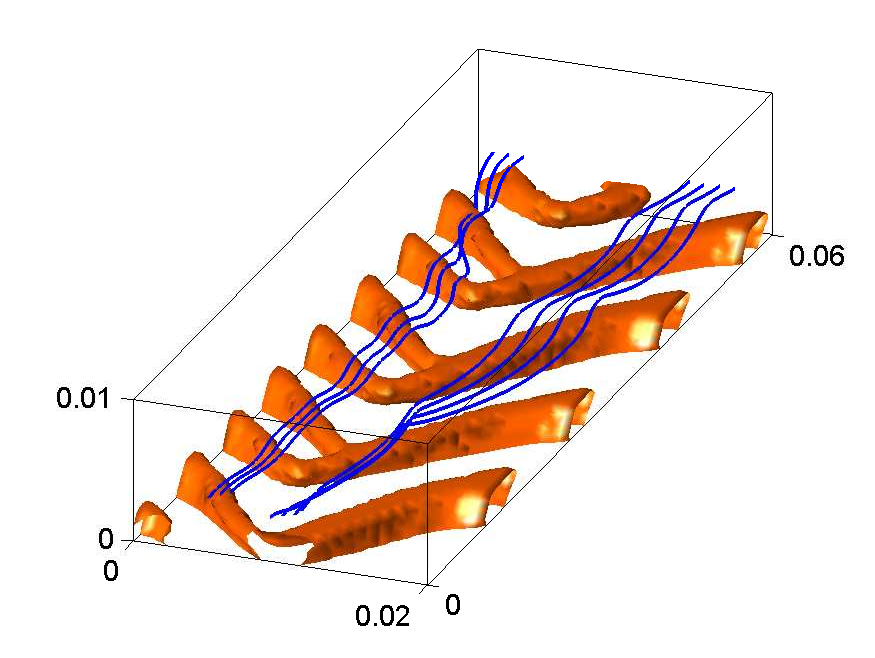
\includegraphics[height=4.3cm]{myharringbonestructure}
    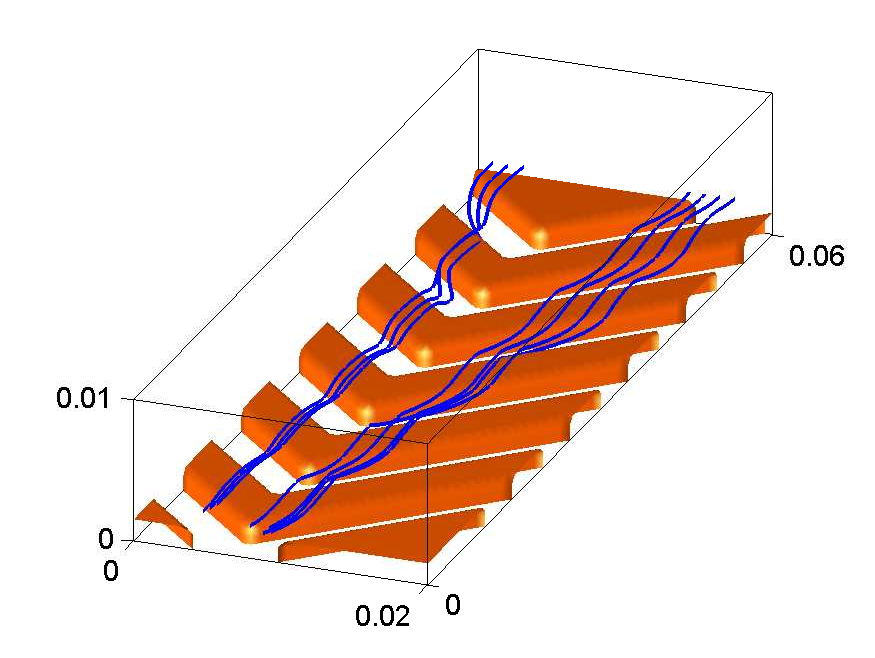
\includegraphics[height=4.3cm]{stroockstructure}
  \end{center}
\end{frame}
%%%%%%%%%%%%%%%%%%%%%%%%%%%%%%%%%%%%%%%%%%%%%%%%%%%%%%%%%%%%%%%%%%%%%%%
\begin{frame}
  \myframetitle{Mixing Lengths}
  \begin{itemize}
  \item Optimal herringbone structure improves mixing length by 30\%,
    optimal 3D structure by 60\%.
  \end{itemize}
  \begin{center}
    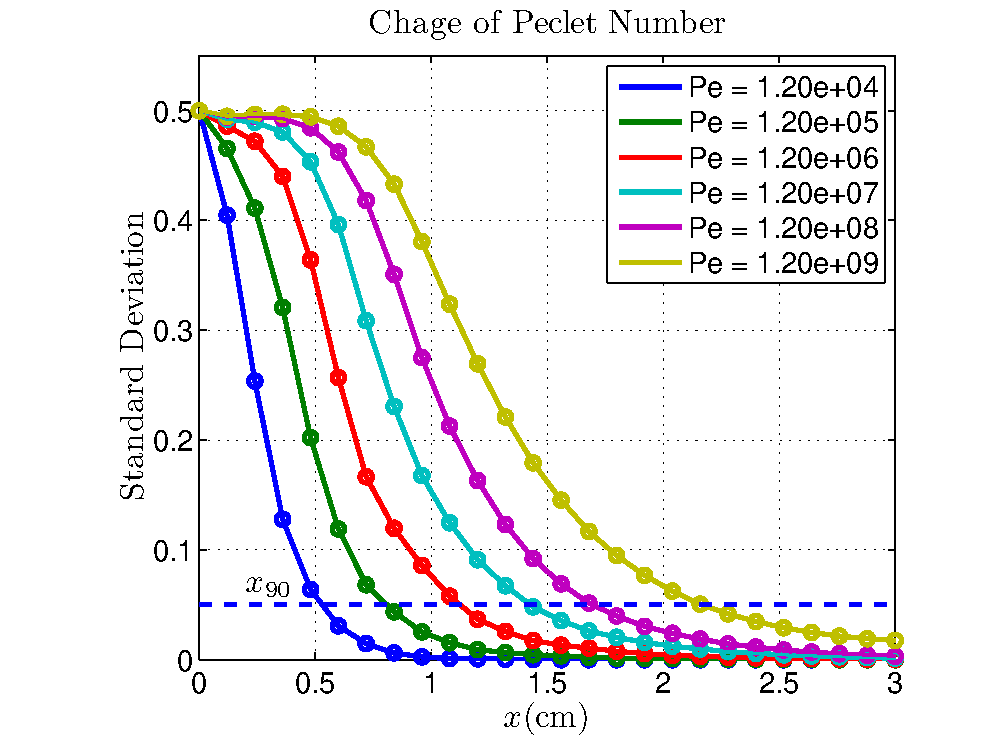
\includegraphics[height=4.4cm]{example2veryPe2}
    \hfill
    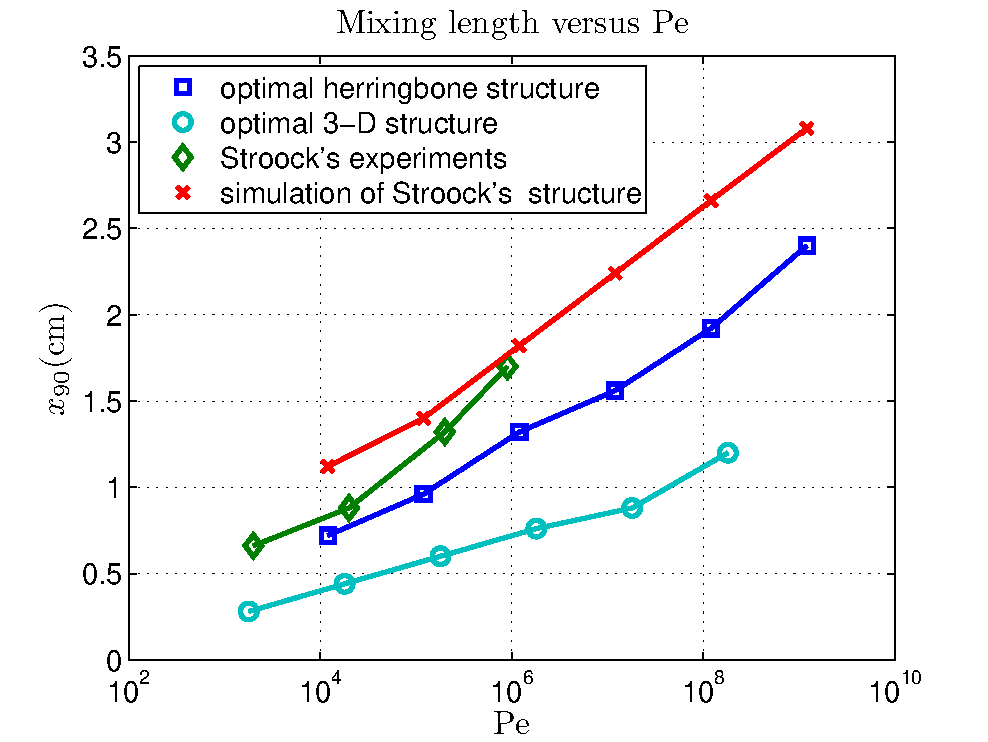
\includegraphics[height=4.4cm]{example2mixinglength2}
  \end{center}
\end{frame}
%%%%%%%%%%%%%%%%%%%%%%%%%%%%%%%%%%%%%%%%%%%%%%%%%%%%%%%%%%%%%%%%%%%%%%%
\begin{frame}
  \myframetitle{Channel Cross-sections}
  \begin{itemize}
  \item 3D structure has lower velocity for same pressure.
    \begin{itemize}
    \item Measure mixing rate by time or distance?
    \end{itemize}
  \end{itemize}
  \begin{center}
    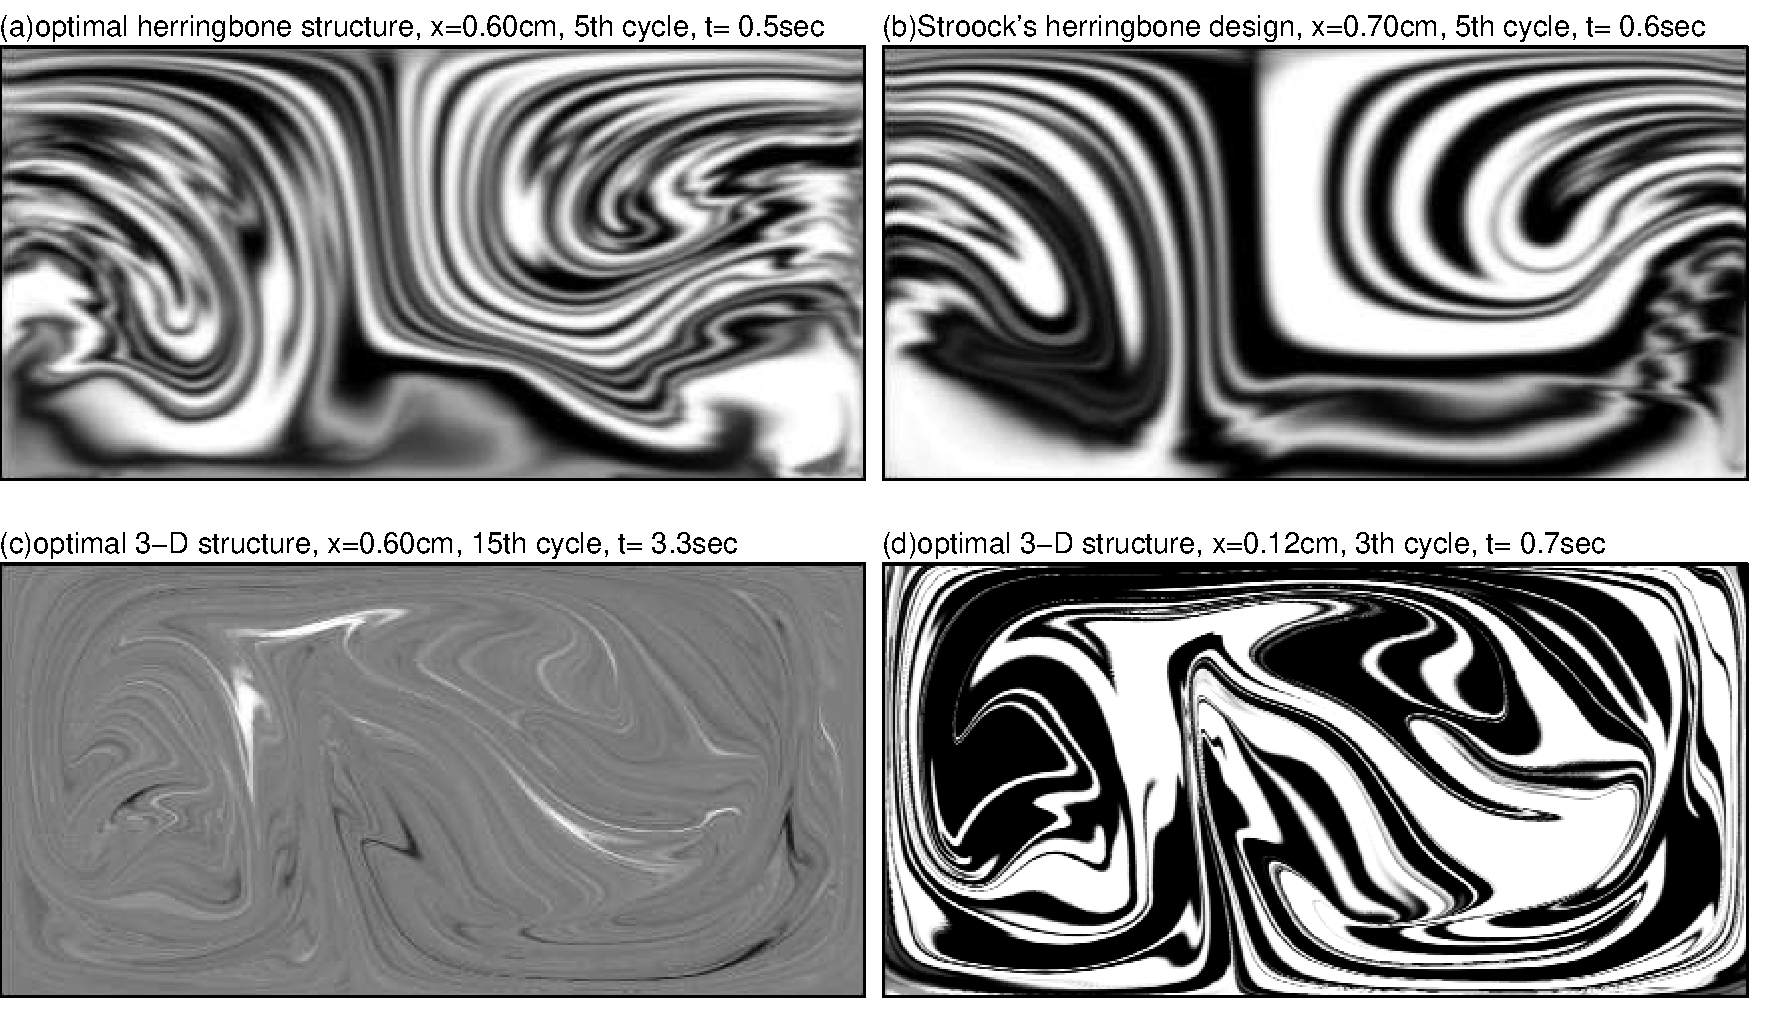
\includegraphics[height=5cm]{example2crosscompare}
  \end{center}
\end{frame}
%%%%%%%%%%%%%%%%%%%%%%%%%%%%%%%%%%%%%%%%%%%%%%%%%%%%%%%%%%%%%%%%%%%%%%%
\begin{frame}
  \myframetitle{Mixing Evolution}
  \begin{itemize}
  \item Why not optimize mixing directly?
    \begin{itemize}
    \item Can't compute the gradient of mixing length.
    \end{itemize}
  \item Can we use Markov Chain mixing properties?
    \begin{itemize}
    \item Mixing rate determined by $\lambda_2$?
    \end{itemize}
  \end{itemize}
  \begin{center}
    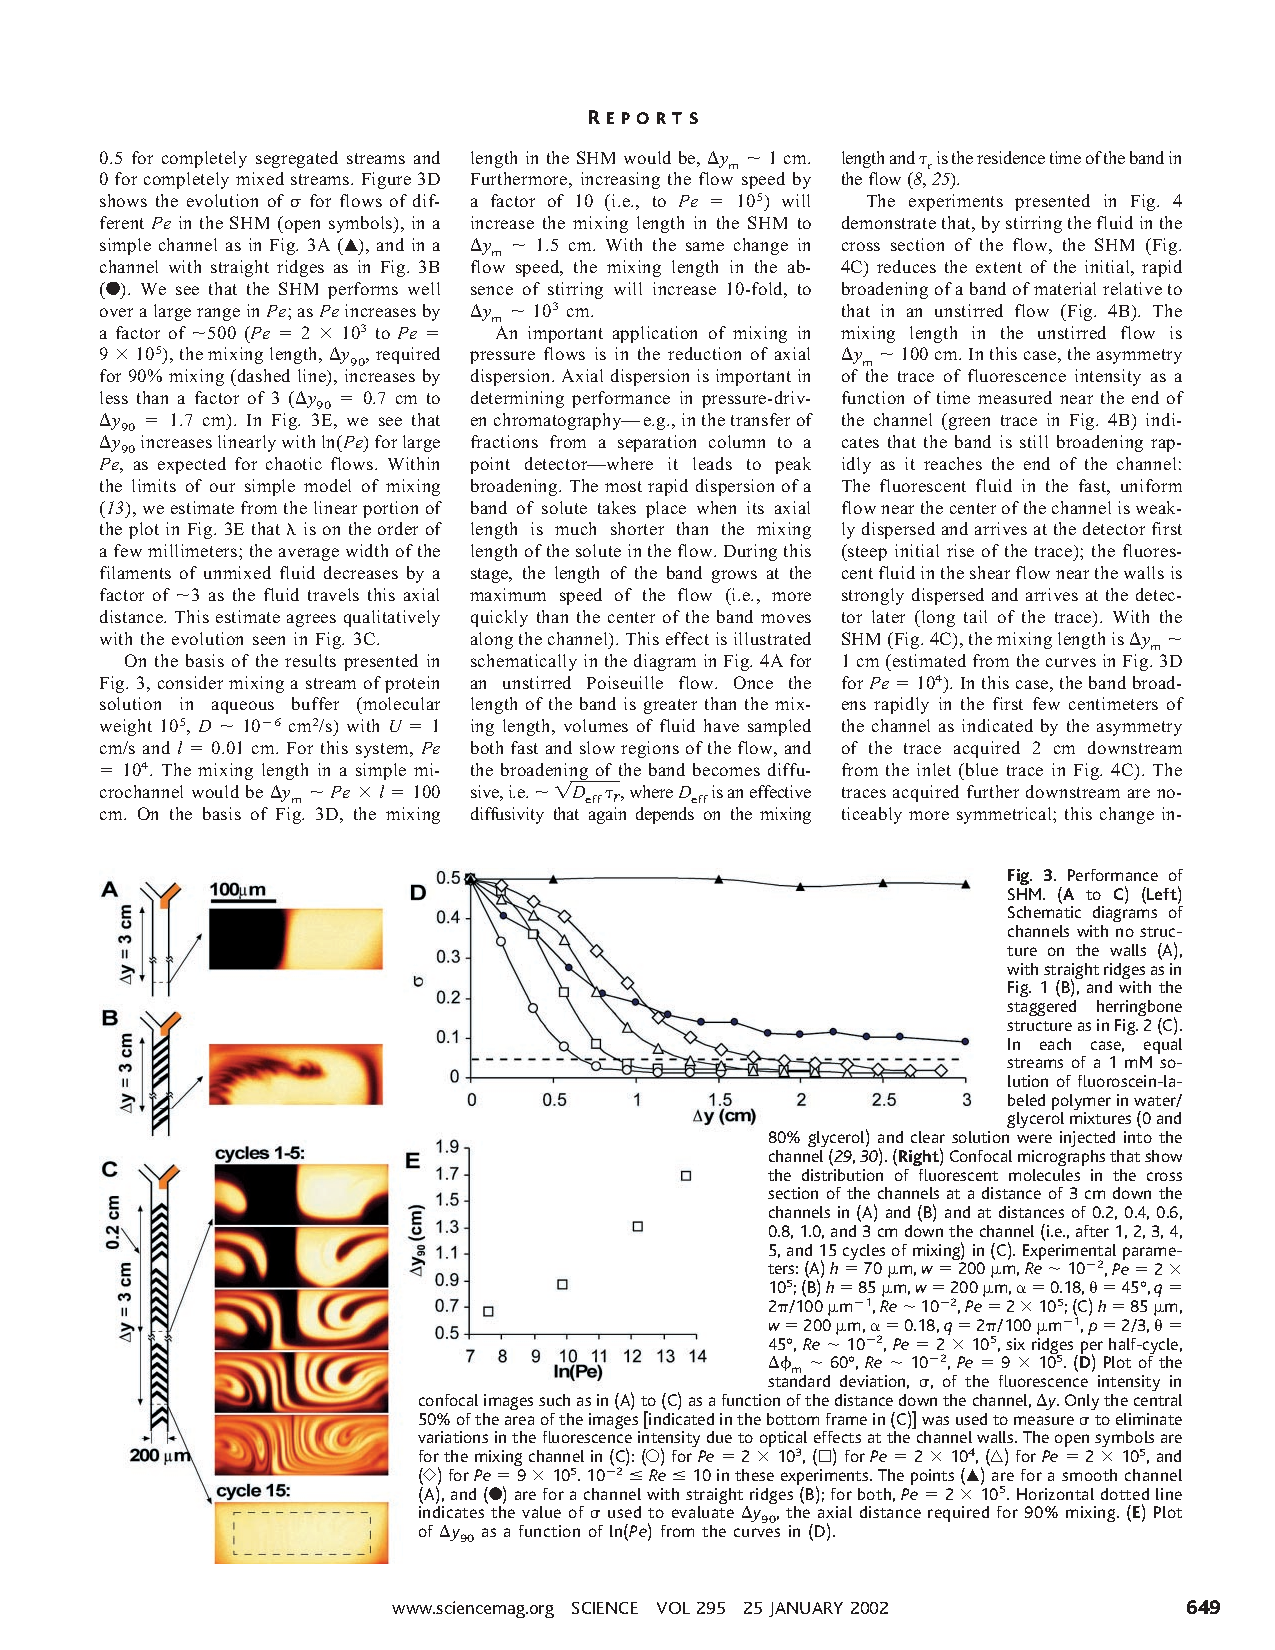
\includegraphics[height=4cm,trim=6.5cm 8.8cm 5cm 14cm,clip=true]{stroock_page3}
  \end{center}
\end{frame}
%%%%%%%%%%%%%%%%%%%%%%%%%%%%%%%%%%%%%%%%%%%%%%%%%%%%%%%%%%%%%%%%%%%%%%%
\begin{frame}
  \myframetitle{GSR Riffle Shuffles in Cards}
  \begin{itemize}
  \item The basic model of riffle shuffles was introduced by Gilbert
    and Shannon (1955) and Reeds (1981).
    \item A deck of $n = 52$ cards is cut into two piles according to
      the binomial distribution so the chance that pile one has $j$
      cards is ${n \choose j}/2^n$.
    \item Then sequentially drop cards from the bottoms of the two piles
      according to the following rule: if at some stage pile one has $A$
      cards and pile two has $B$ cards, drop the next card from pile one
      with probability $A/(A+B)$.
    \item This is continued until the two piles are exhausted.
    \item Markov chain with $n! = 52! = 8 \times 10^{67}$ states.
  \end{itemize}
\end{frame}
%%%%%%%%%%%%%%%%%%%%%%%%%%%%%%%%%%%%%%%%%%%%%%%%%%%%%%%%%%%%%%%%%%%%%%%
\begin{frame}
  \myframetitle{GSR Riffle Shuffles in Cards}
  \begin{itemize}
  \item Question: How many shuffles to randomize $52$ cards?
    \begin{center}
      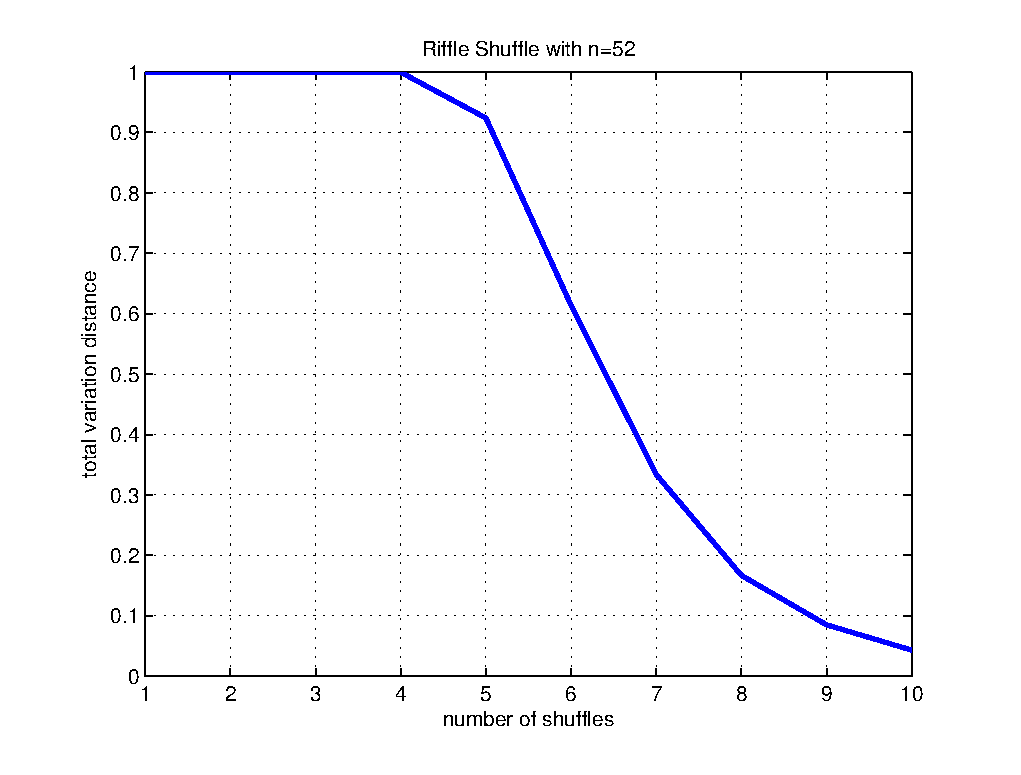
\includegraphics[width=0.55\textwidth,trim=1cm 1cm 0cm 0cm]{riffleshuffle}
    \end{center}
  \item Answer: 7
  \item Aldous and Diaconis, 1986
  \end{itemize}
\end{frame}
%%%%%%%%%%%%%%%%%%%%%%%%%%%%%%%%%%%%%%%%%%%%%%%%%%%%%%%%%%%%%%%%%%%%%%%
\begin{frame}
  \myframetitle{Cutoff in Markov Chains}
  \begin{itemize}
  \item Finite set $\Omega$ with ``metric'' $D$ on
    probability measures $\mu$, $\nu$, so that
    $D(\mu,\nu)$ such that 
    \begin{enumerate}
    \item $D(\mu,\nu)\in [0,1]$
    \item $\max_{\Omega,\mu,\nu} D(\mu,\nu) = 1$
    \item $D(\mu,\nu)=0$ if and only if $\mu=\nu$
    \end{enumerate}
  \item Sequence of probability spaces $(\Omega_n,\nu_n)$,
    $n=1,2,\ldots$, each with a sequence of probability measures
    $\mu^k_n$, $l=0,1,\ldots$, such that
    \begin{align*}
      \lim_{k \rightarrow \infty} D(\mu^k_n,\nu_n)=0
    \end{align*}
  \item Think of $n$ as dimension of a Markov Chain, $k$ as iteration
    number, $\mu^0_n$ as initial distribution, $\nu_n$ as invariant
    distribution.
  \item Examples: riffle shuffle of $n$ cards, random walk on
    $n$-dimensional hypercube, Ehrenfest's urn with $n$ balls, \ldots
  \end{itemize}
\end{frame}
%%%%%%%%%%%%%%%%%%%%%%%%%%%%%%%%%%%%%%%%%%%%%%%%%%%%%%%%%%%%%%%%%%%%%%%
\begin{frame}
  \myframetitle{Cutoff in Markov Chains}
  \begin{itemize}
  \item \textbf{Definition:} (Diaconis) A family $(\Omega_n,\nu_n,
    (\mu^k_n)_{k=0,1,...})_{n=1,2,...}$ presents a $D$-cutoff if there
    exists a sequence $(t_n)$ of positive reals such that, for any
    $\epsilon \in(0,1)$,
    \begin{enumerate}
    \item $\lim_{k \rightarrow \infty}D(\mu^{k_n}_n,\nu_n) = 0 \mbox{ if }
      k_n>(1+\epsilon)t_n$
    \item $\lim_{k \rightarrow \infty}D(\mu^{k_n}_n,\nu_n) = 1 \mbox{ if }
      k_n<(1-\epsilon)t_n $
    \end{enumerate}
    \begin{center}
      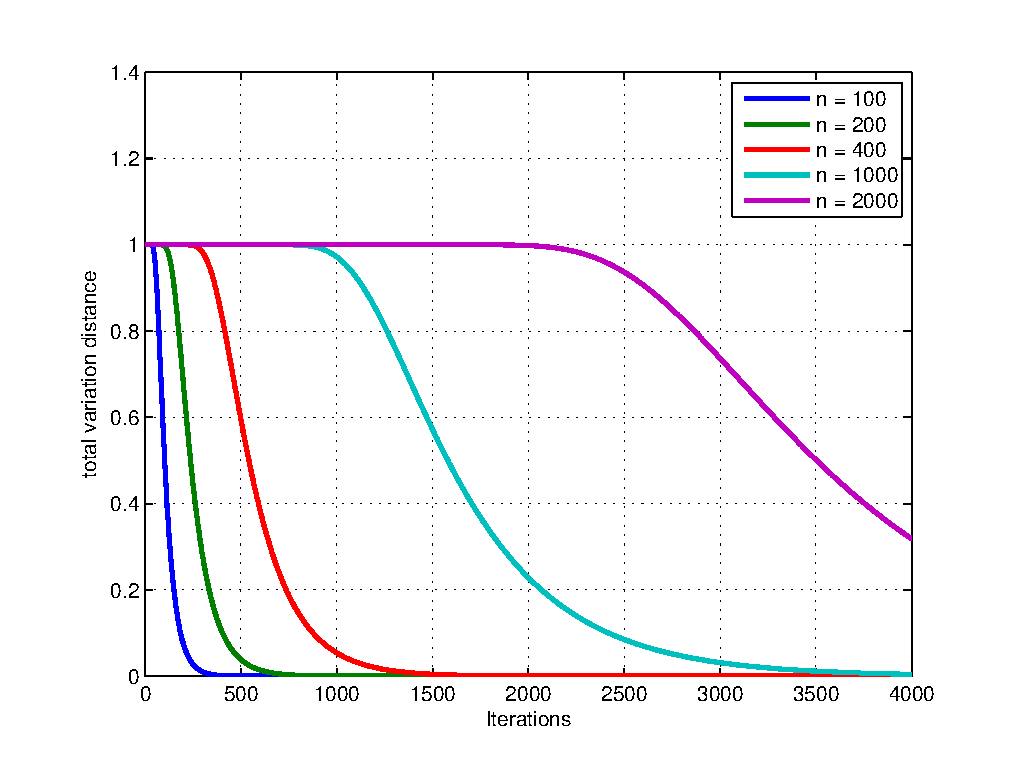
\includegraphics[width=0.43\textwidth,trim=1cm 1cm 0cm 0cm]{rdwalk}
      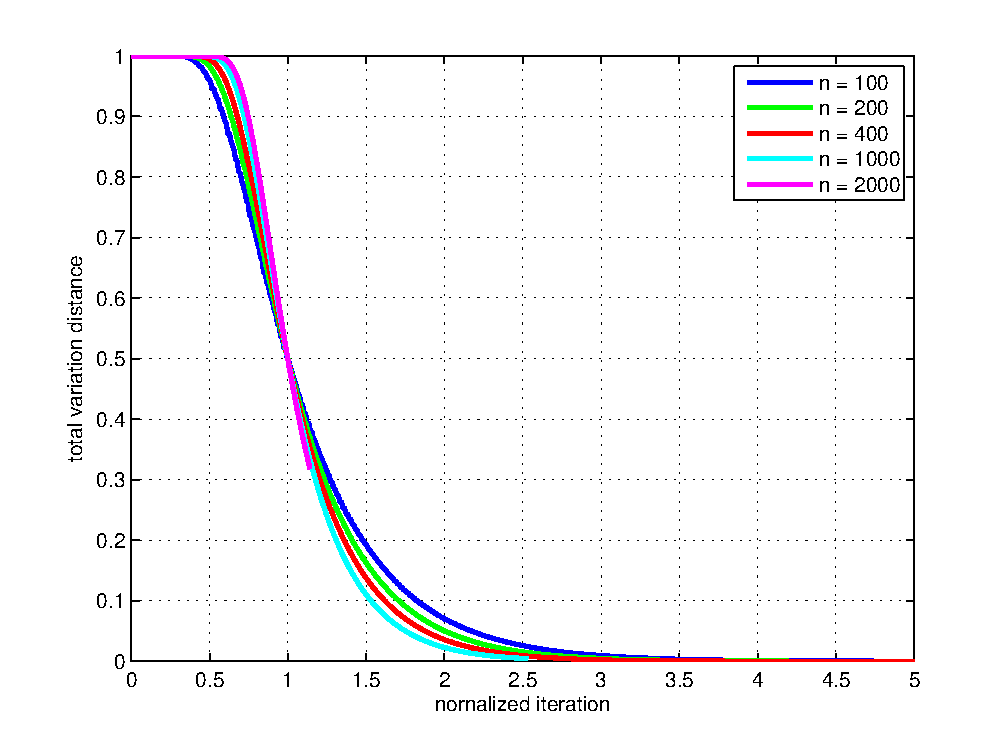
\includegraphics[width=0.43\textwidth,trim=1cm 1cm 0cm 0cm]{rdwalkn}
    \end{center}
  \end{itemize}
\end{frame}
%%%%%%%%%%%%%%%%%%%%%%%%%%%%%%%%%%%%%%%%%%%%%%%%%%%%%%%%%%%%%%%%%%%%%%%
\begin{frame}
  \myframetitle{Cutoff in Chaotic Maps}
  \begin{itemize}
  \item Are we seeing cutoff in chaotic mixing?
    \begin{itemize}
    \item Numerical supporting evidence in 2D and higher.
    \item Provable for some 1D maps and certain initial conditions.
    \end{itemize}
  \item Non-convex mixing long recognized in chaotic mixing literature.
    \begin{itemize}
    \item Super-exponential mixing phase.
    \end{itemize}
  \item Both primal and dual cutoffs:
    \begin{itemize}
    \item Perron-Frobenius evolution of a narrow probability
      distribution to the invariant distribution.
    \item Koopman evolution of a low frequency initial function to a
      high frequency function and then constant.
    \end{itemize}
  \end{itemize}
\end{frame}
%%%%%%%%%%%%%%%%%%%%%%%%%%%%%%%%%%%%%%%%%%%%%%%%%%%%%%%%%%%%%%%%%%%%%%%
\begin{frame}
  \myframetitle{Standard Map}
  \begin{itemize}
  \item Standard map on the unit square:
    \begin{align*}
      x_1 &\leftarrow x_1 + x_2 + \epsilon \sin 2\pi x_1 \text{ (mod 1)} \\
      x_2 &\leftarrow x_2 + \epsilon \sin 2\pi x_1 \text{ (mod 1)} \\
    \end{align*}
  \end{itemize}
  \vspace{-1cm}
  \begin{center}
    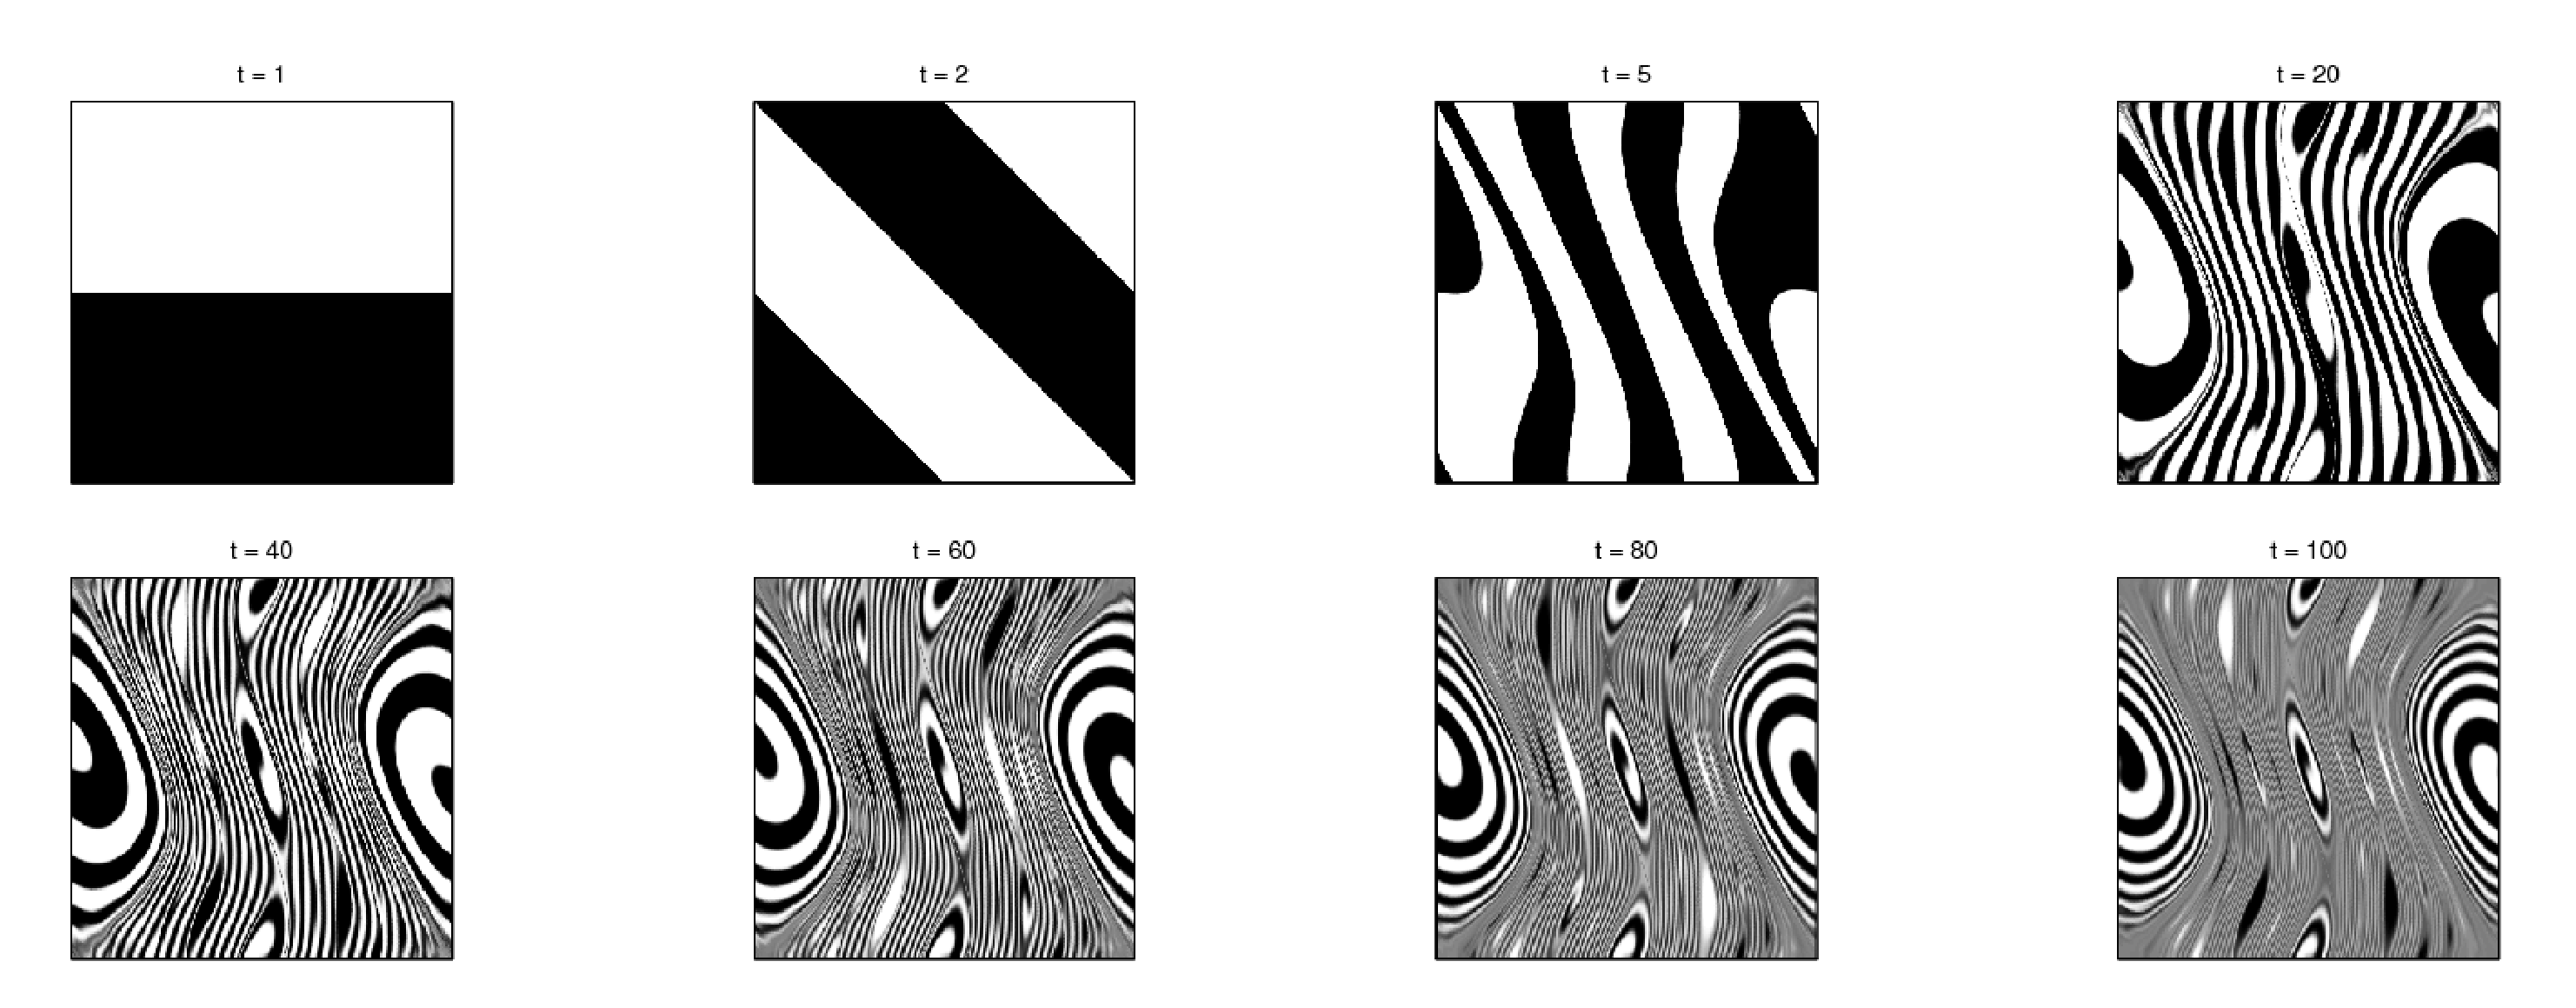
\includegraphics[width=0.8\textwidth]{Standardmapexample_crop}
  \end{center}
\end{frame}
%%%%%%%%%%%%%%%%%%%%%%%%%%%%%%%%%%%%%%%%%%%%%%%%%%%%%%%%%%%%%%%%%%%%%%%
\begin{frame}
  \myframetitle{Standard Map}
  \begin{itemize}
  \item Approximate Perron-Frobenius operator by Markov Chain on $n
    \times n$ grid:
  \end{itemize}
  \begin{center}
    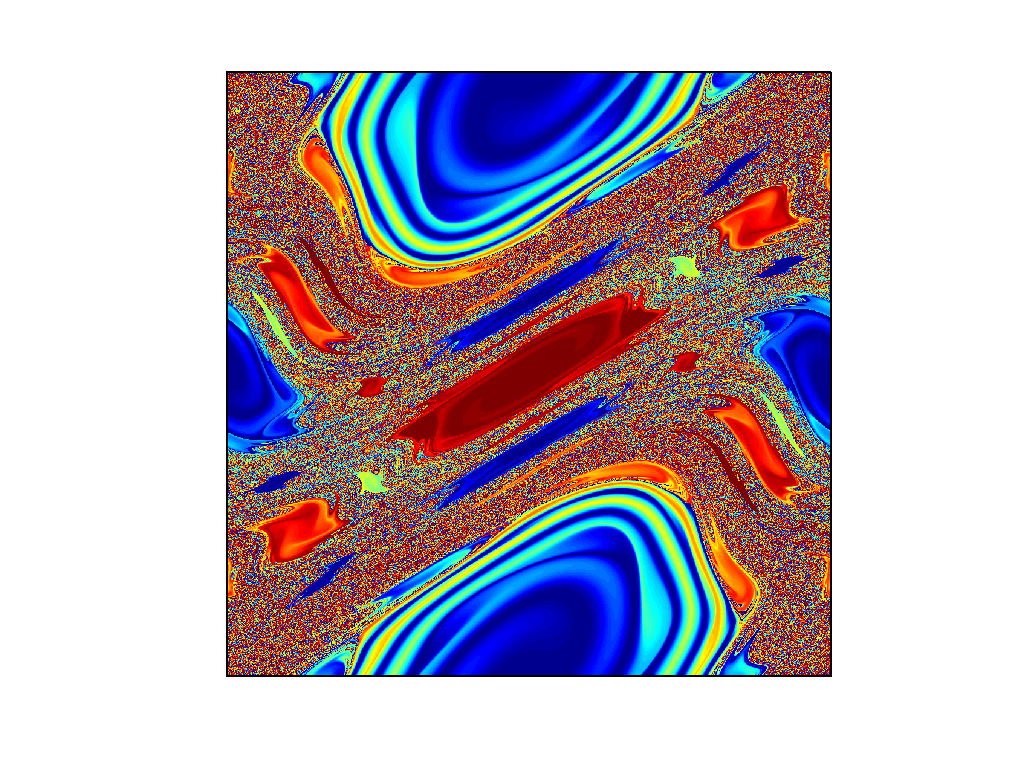
\includegraphics[height=3cm,trim=3.5cm 1.5cm 3cm 1cm]{standardmapsimuexact}
    \hspace{1cm}
    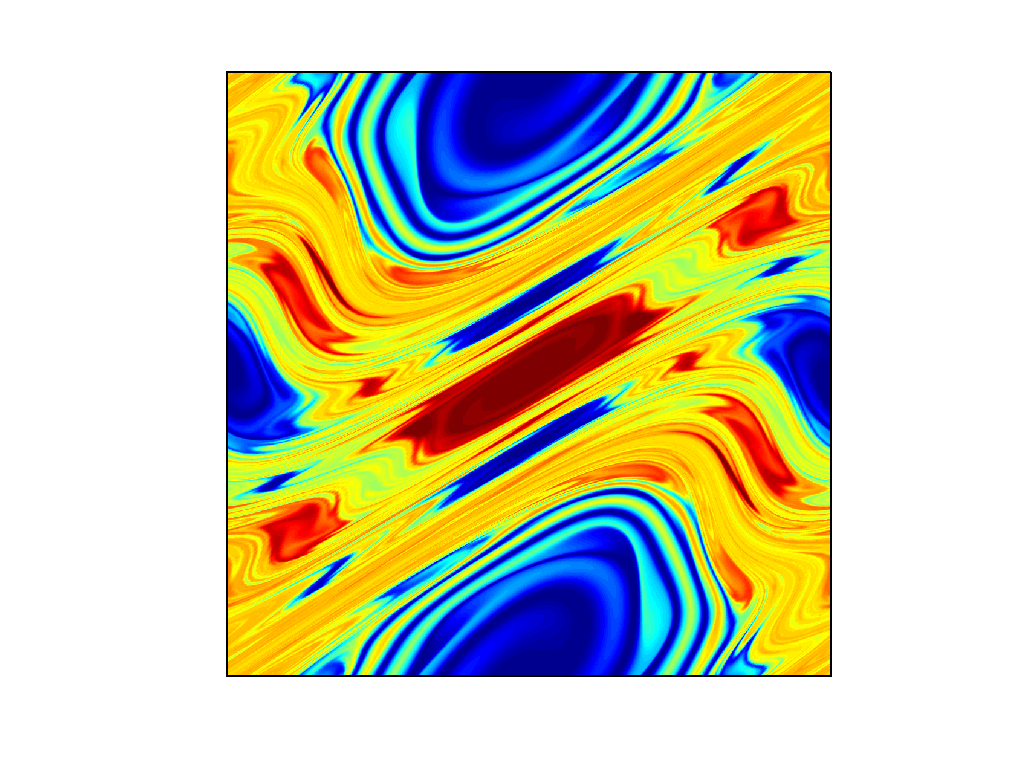
\includegraphics[height=3cm,trim=3.5cm 1.5cm 3cm 1cm]{standardmapsimumarkov}
  \end{center}
  \begin{itemize}
  \item Compute to $n = 80000$
    \begin{itemize}
      \item[$\Longrightarrow$] Markov Chain with $64 \times 10^8$
        states (riffle shuffle has $8 \times 10^{67}$).
      \item[$\Longrightarrow$] $50\,\text{GB}$ to store a probability
        distribution.
    \end{itemize}
  \end{itemize}
\end{frame}
%%%%%%%%%%%%%%%%%%%%%%%%%%%%%%%%%%%%%%%%%%%%%%%%%%%%%%%%%%%%%%%%%%%%%%%
\begin{frame}
  \myframetitle{Cutoff in the Standard Map}
  \begin{itemize}
  \item Simulations show cutoff for Koopman evolution.
  \item $\epsilon = 0.3$, initial condition $c^0(x) = \cos(2\pi x_2)$.
  \end{itemize}
  \begin{center}
    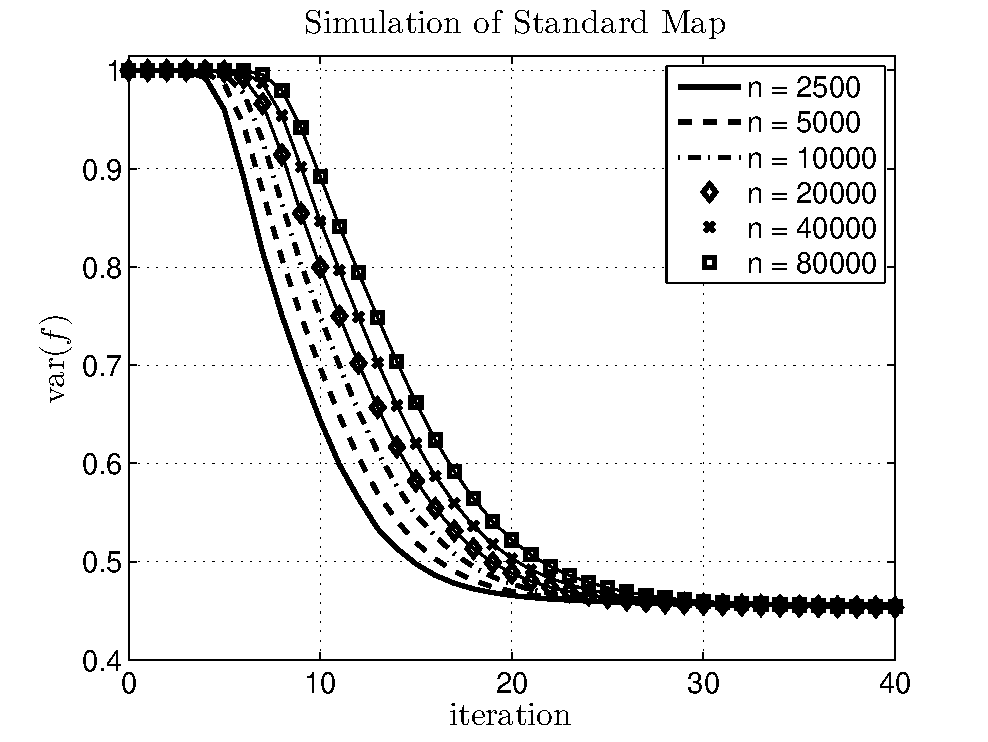
\includegraphics[width=5.7cm]{standardmapcutoff}
    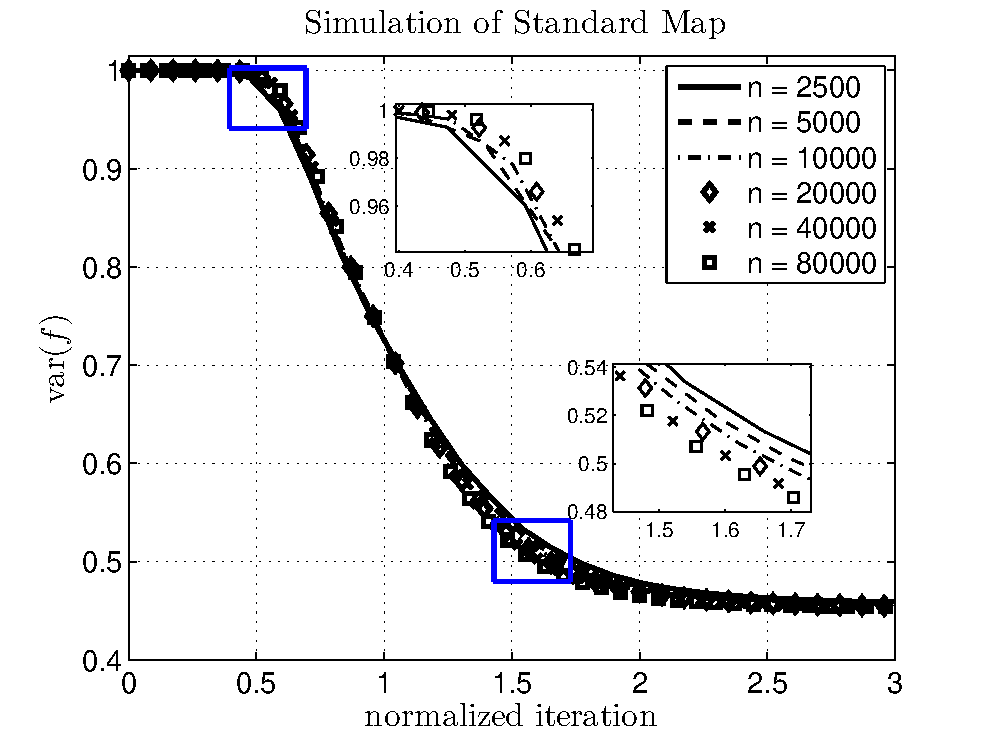
\includegraphics[width=5.7cm]{standardmapcutoffn}
  \end{center}
  \begin{itemize}
  \item Only looks slow because we can't simulate large systems.
  \end{itemize}
\end{frame}
%%%%%%%%%%%%%%%%%%%%%%%%%%%%%%%%%%%%%%%%%%%%%%%%%%%%%%%%%%%%%%%%%%%%%%%
\begin{frame}
  \myframetitle{Cutoff in the Standard Map}
  \begin{itemize}
  \item Measure distance to sharp transition:
    \begin{equation*}
      c^{\infty}(x) = \begin{cases}
        M, &\text{if } x < 1, \\
        m, &\text{otherwise}
      \end{cases}
      \qquad
      \Delta^l = \int_0^l | c^k(x)-c^{\infty}(x)|\,dx
    \end{equation*}
  \end{itemize}
  \begin{center}
    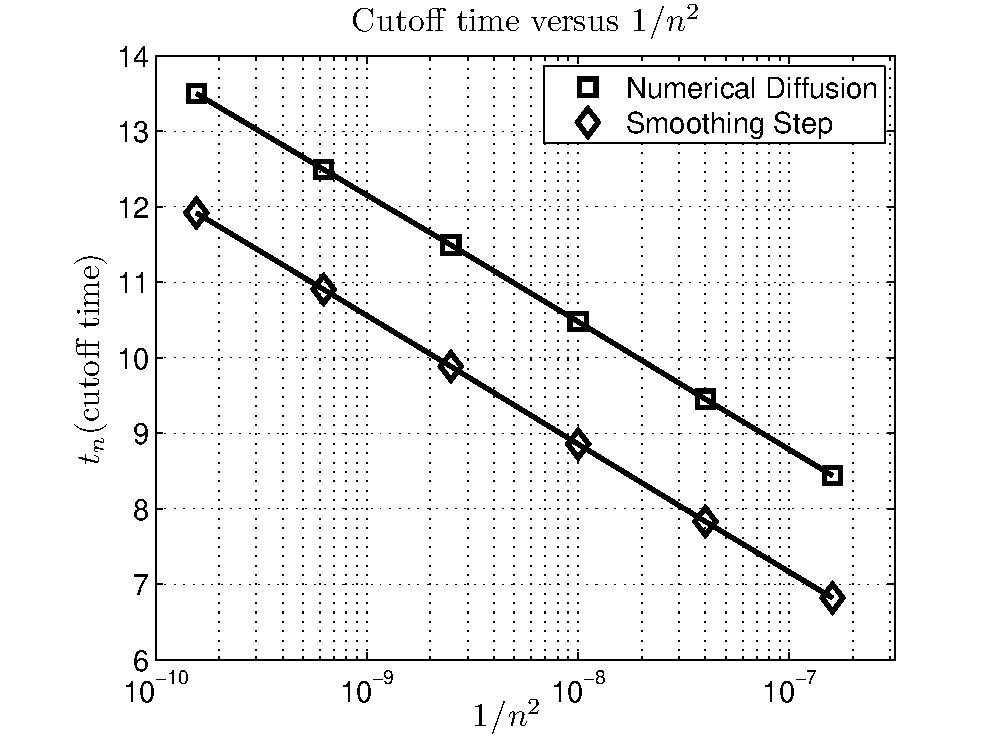
\includegraphics[width=5cm]{cutofftimevsD}
    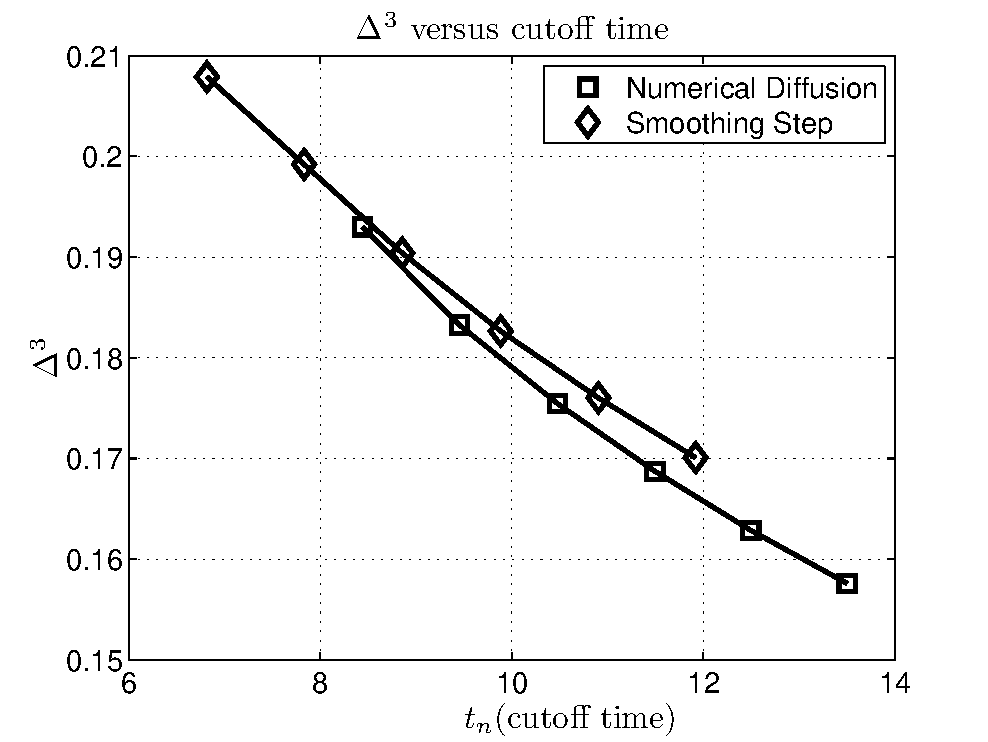
\includegraphics[width=5cm]{areavscutofftime}
  \end{center}
\end{frame}
%%%%%%%%%%%%%%%%%%%%%%%%%%%%%%%%%%%%%%%%%%%%%%%%%%%%%%%%%%%%%%%%%%%%%%%
\begin{frame}
  \myframetitle{Cutoff in 1D Maps}
  \begin{itemize}
  \item Baker's map on $T^2$
    \begin{equation*}
      f(x_1,x_2) = 
      \begin{cases}
        (2x_1,\frac{1}{2}x_2) \text{ mod } 1,
        & \text{if } 0 \le x_1 < \frac{1}{2} \\
        (2x_1,\frac{1}{2}(x_2+1)) \text{ mod } 1,
        & \text{if } \frac{1}{2} \le x_1 < 1
      \end{cases}
    \end{equation*}
  \item Initial condition $c^0(x)= \sqrt{\pi} \cos(2 \pi x_2)$,
    diffusion operator with diffusivity $D$ is applied after every
    iteration.
  \end{itemize}
  \begin{center}
    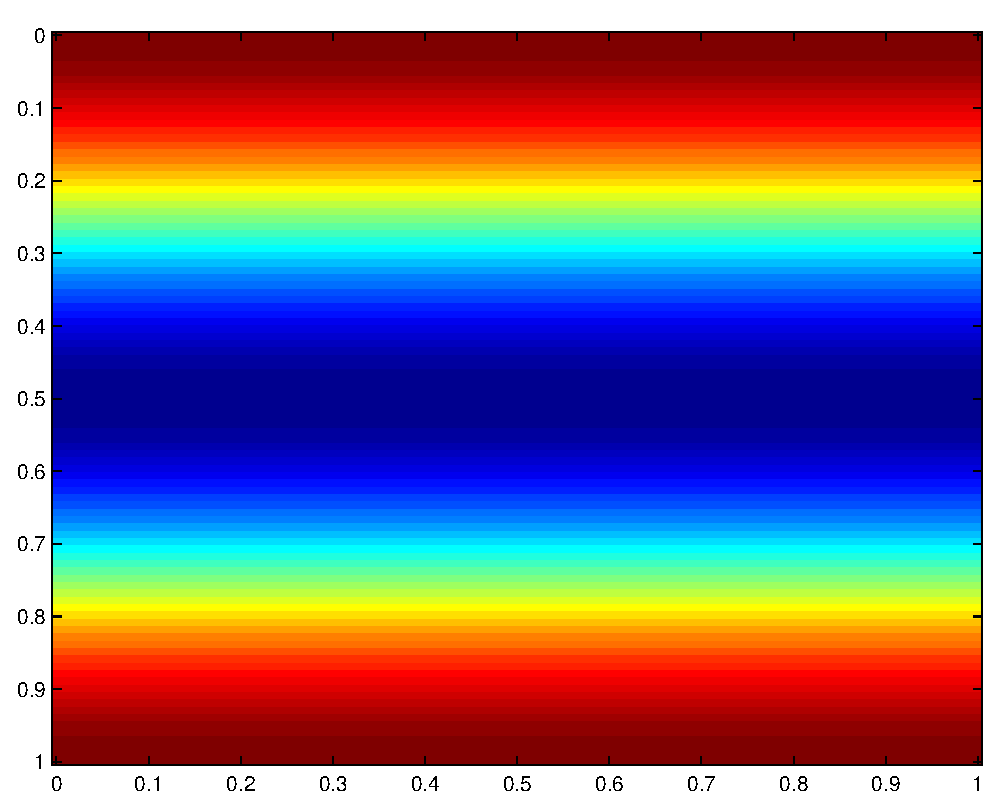
\includegraphics[width=0.3\textwidth]{baker1}
    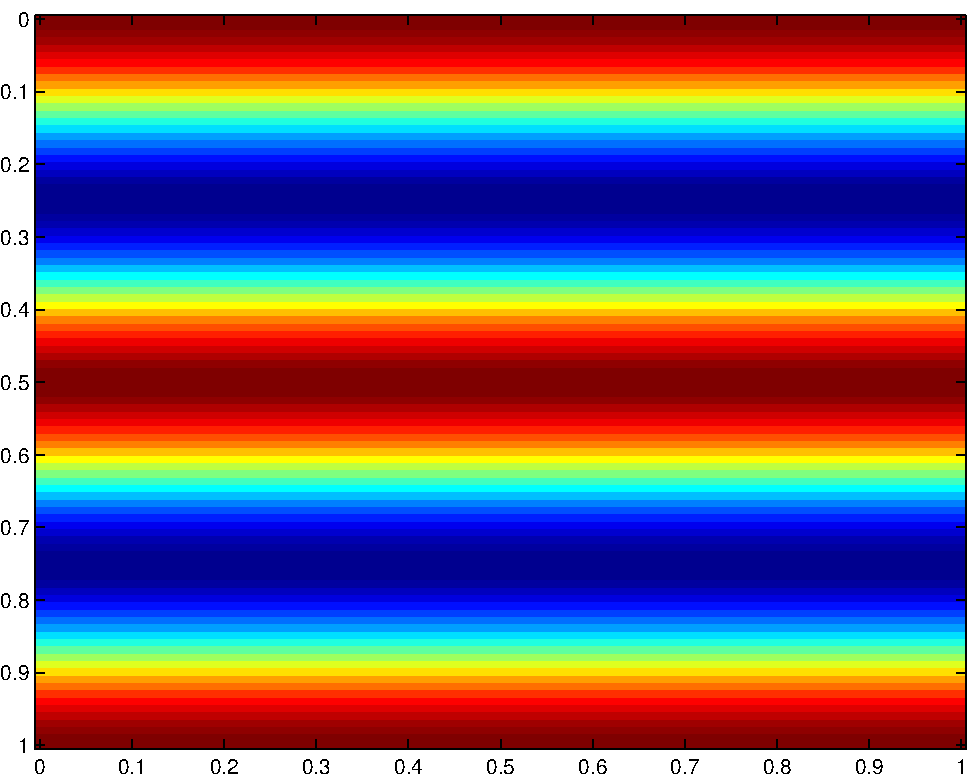
\includegraphics[width=0.3\textwidth]{baker2}
    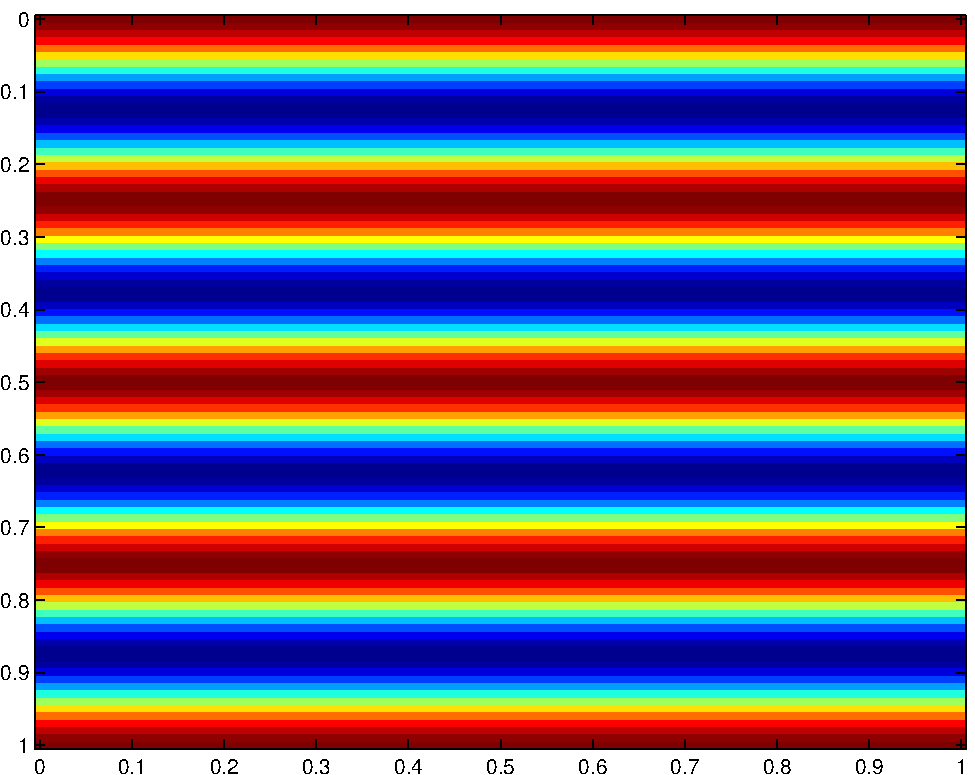
\includegraphics[width=0.3\textwidth]{baker3}
  \end{center}
\end{frame}
%%%%%%%%%%%%%%%%%%%%%%%%%%%%%%%%%%%%%%%%%%%%%%%%%%%%%%%%%%%%%%%%%%%%%%%
\begin{frame}
  \myframetitle{Cutoff in Baker's Map}
  \begin{itemize}
  \item Analytically solvable:
    \begin{align*}
      c^k(x) &= \sqrt{\pi} e^{-4 \pi^2 D 2 ^{2 k}}\cos(2 \pi 2^k x_2)
      \text{ for } k = 1,2,\ldots \\
      \|c^k(x)\|_2 &= e^{-4 \pi^2 D 2^{2 k}}
    \end{align*}
  \item Cutoff as diffusion $D = 1/n$ decreases:
    \begin{center}
      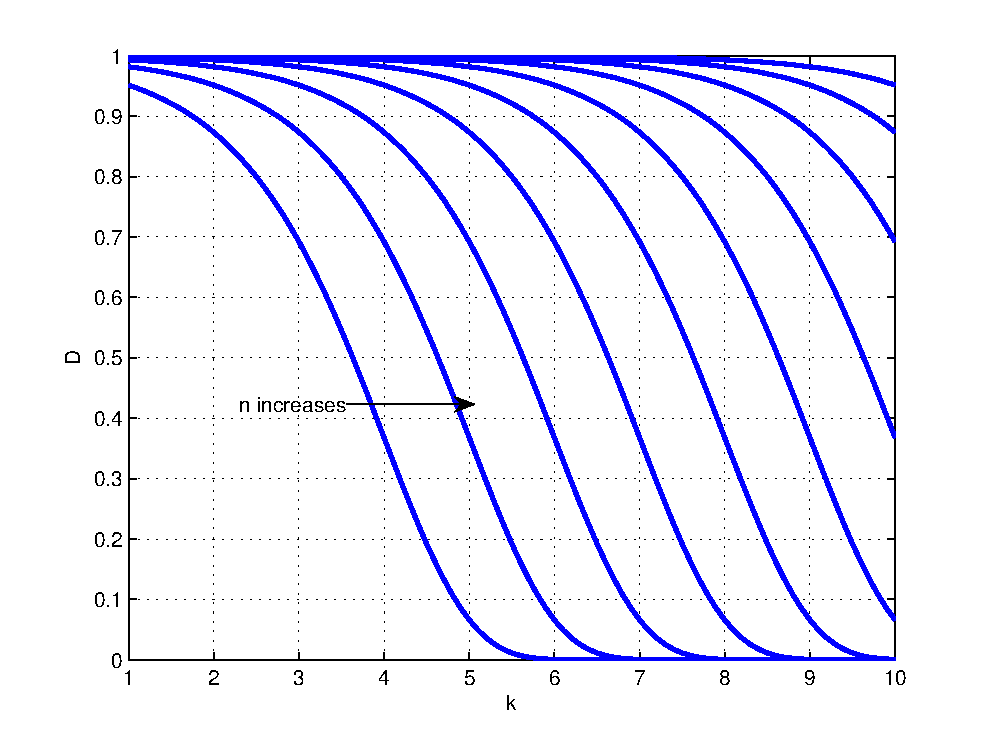
\includegraphics[width=5cm]{democutoff1}
      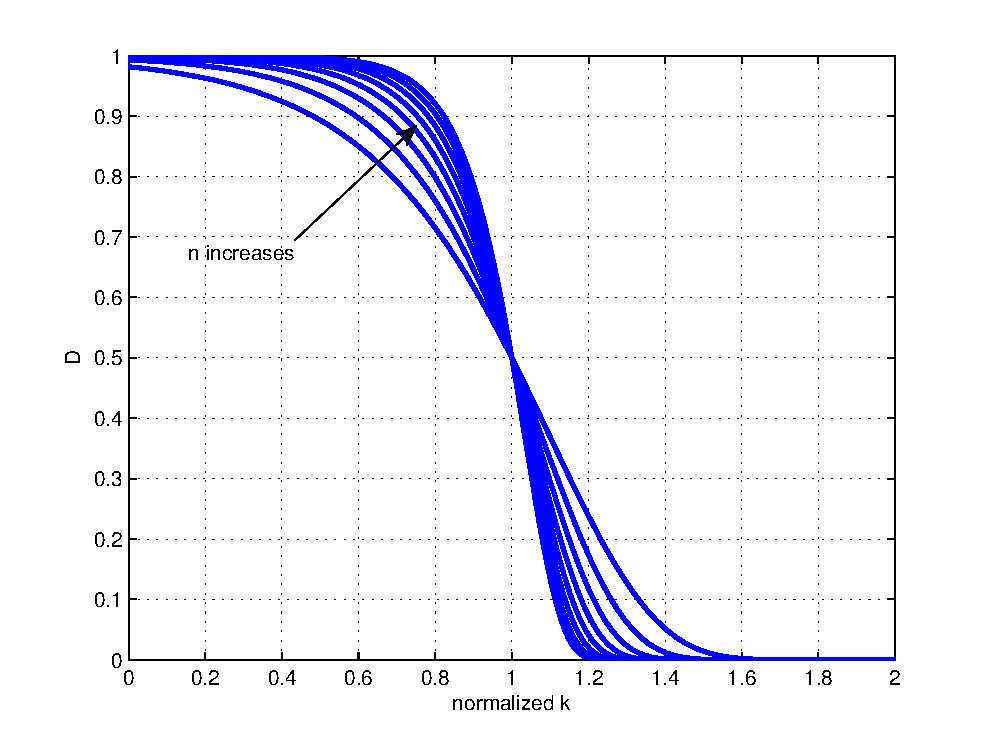
\includegraphics[width=5cm]{democutoff1n}
    \end{center}
  \end{itemize}
\end{frame}
%%%%%%%%%%%%%%%%%%%%%%%%%%%%%%%%%%%%%%%%%%%%%%%%%%%%%%%%%%%%%%%%%%%%%%%
\begin{frame}
  \myframetitle{Symbolic Dynamics}
  \begin{itemize}
    \item Deterministic symbolic dynamics:
      \begin{itemize}
      \item Partition phase space into $L \cup R$.
      \item For each initial condition $x_0$ a map $x \mapsto f(x)$
        generates a symbol sequence: $x_0 \sim (L, L, R, L, R, L, R,
        R, L, \ldots)$.
      \item The symbol sequence for the initial condition $f(x_0)$ is
        the shift of that for $x_0$ itself: $f(x_0) \sim (L, R, L, R,
        L, R, R, L, \ldots)$.
      \item Chaotic maps $f(x)$ are homeomorphic to the shift map on
        space of symbol sequences.
      \end{itemize}
    \item Stochastic symbol sequences:
      \begin{itemize}
      \item A stochastic symbol sequence $(\delta_0, \delta_1,
        \delta_2, \ldots)$ gives $\operatorname*{Prob}(f^k(x) \in L) =
        \delta_k \in [0,1]$.
      \item Defines measure $\omega$ on state space by assuming
        independence of $f^k(x)$ and $f^{k+1}(x)$.
      \end{itemize}
  \end{itemize}
\end{frame}
%%%%%%%%%%%%%%%%%%%%%%%%%%%%%%%%%%%%%%%%%%%%%%%%%%%%%%%%%%%%%%%%%%%%%%%
\begin{frame}
  \myframetitle{Cutoff with Symbolic Dynamics}
  \begin{itemize}
  \item \textbf{Theorem:} Define $\omega_n^0$ by $(\delta_0, \delta_1,
    \ldots)$ with $\delta_i = \max\{\frac{1}{2}+\epsilon_n r_n^i,1\}$
    for $\epsilon_n = \sqrt{n(1-r_n)/4}$ and $r_n = e^{-\frac{2}{n}}$.
    Let $k = \frac{1}{4}n\log{n}+cn $, then
    \begin{equation*}
      \operatorname*{erf}\left(\sqrt{\frac{n}{8}}e^{-\frac{2k}{n}-1}  \right)
      \le |\omega^k_n - \bar{\omega}|_{TV}
      \le \operatorname*{erf}\left(\sqrt{\frac{n}{8}}e^{-\frac{2k}{n}}  \right)
    \end{equation*}
  \end{itemize}
  \begin{center}
    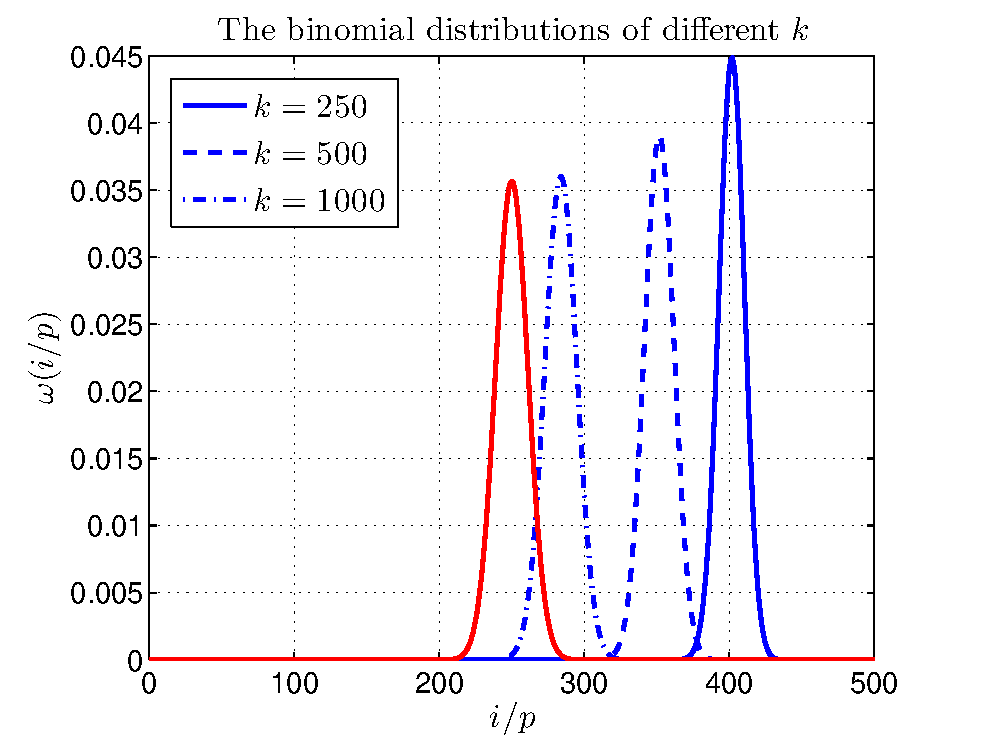
\includegraphics[height=3cm]{deltaMexample2a}
    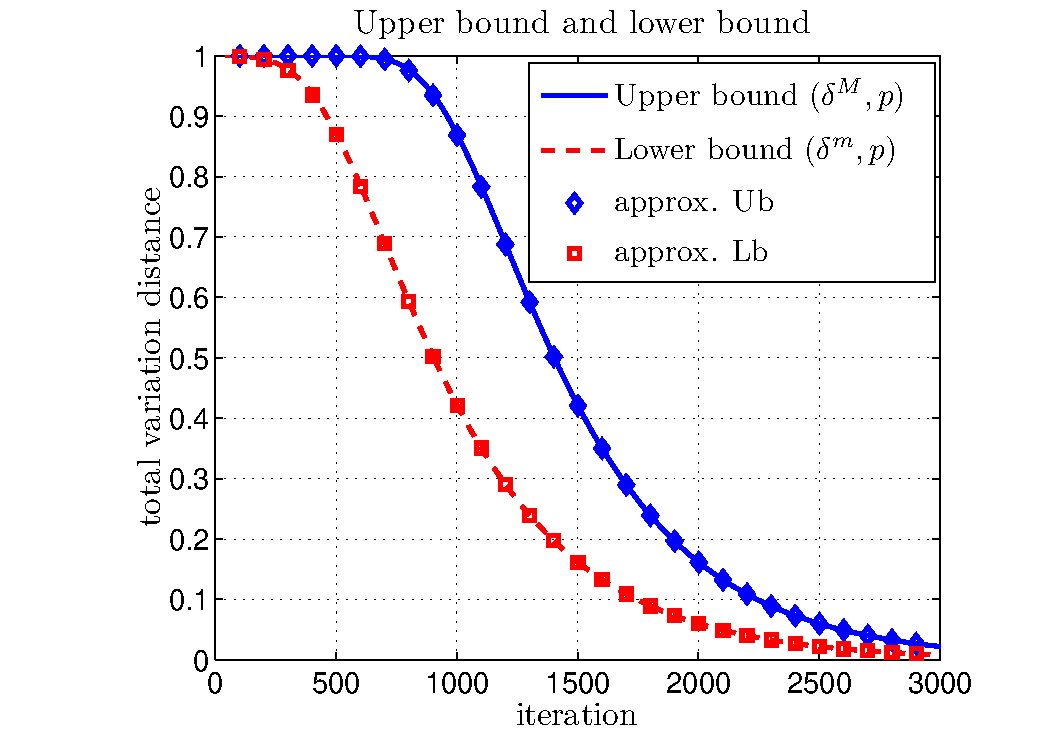
\includegraphics[height=3cm]{deltaMexample2b}
  \end{center}
  \begin{itemize}
  \item Having symbolic dynamics is sufficient to produce cutoff.
  \end{itemize}
\end{frame}
%%%%%%%%%%%%%%%%%%%%%%%%%%%%%%%%%%%%%%%%%%%%%%%%%%%%%%%%%%%%%%%%%%%%%%%
\begin{frame}
  \myframetitle{Concluding Thoughts}
  \begin{itemize}
  \item Universal cause of cutoff in fluids and chaotic maps.
    \begin{itemize}
    \item Exponential growth in interface length (stretching and
      folding) with diffusion.
    \end{itemize}
  \item Engineering and scientific implications.
    \begin{itemize}
    \item Critical mixing time/distance.
    \item Microfluidic channels, ocean circulation mixing, \ldots
    \item Only relevant for large separation between transport and
      diffusion length-scales.
    \end{itemize}
  \item References:
    \begin{itemize}
    \item T.-C. Liang and M. West [2007] Optimized mixing in
      microfluidic channels
    \item T.-C. Liang and M. West [2007] Numerical evidence of cutoffs
      in chaotic mixing
    \item T.-C. Liang and M. West [2007] The cutoff phenomenon and
      mixing properties of chaotic maps
    \end{itemize}
  \end{itemize}
\end{frame}
%%%%%%%%%%%%%%%%%%%%%%%%%%%%%%%%%%%%%%%%%%%%%%%%%%%%%%%%%%%%%%%%%%%%%%%
\begin{frame}
  \myframetitle{Bibliography: Cutoff Phenomenon}
  \begin{itemize}
    % cutoff is firstly named
  \item D. Aldous and P. Diaconis [1986] Shuffling cards and stopping
    times
  \item P. Diaconis, R.L. Graham and J.A. Morrison [1990] Asymptotic
    Analysis of a Random Walk on a Hypercube with Many Dimensions
  \item P. Diaconis [1996] The cutoff phenomena in finite Markov
    Chains
    % Good review
  \item P. Diaconis [2001] Mathematical developments from the analysis
    of riffle shuffling
  \item L. Saloff-Coste [2001] Lectures on probability theory and statistics
  \item P.  Diaconis [2005] Separation cut-offs for death and birth
    chains
  \end{itemize}
\end{frame}
%%%%%%%%%%%%%%%%%%%%%%%%%%%%%%%%%%%%%%%%%%%%%%%%%%%%%%%%%%%%%%%%%%%%%%%
\begin{frame}
  \myframetitle{Bibliography: Chaotic Map Mixing}
  \begin{itemize}
  \item D.R. Fereday, P.H. Haynes, A. Wonhas, and J.C. Vassilicos
    [2002] Scalar variance decay in chaotic advection and
    Batchelor-regime turbulence
    % studies of modified Arnold's cat map
  \item J.-L. Thiffeault and S. Childress [2003] Chaotic mixing in a
    torus map
  \item P.H. Haynes and J. Vanneste [2003] What controls the decay of
    passive scalars in smooth flows?
  \item J.-L. Thiffeault [2004] Scalar decay in chaotic mixing
    % this guy runs 60kx60k simulation
  \item Y.-K. Tsang, T.M. Antonsen, Jr. and E. Ott [2005] Exponential
    decay of chaotically advected passive scalars in the zero
    diffusivity limit
  \end{itemize}
\end{frame}
%%%%%%%%%%%%%%%%%%%%%%%%%%%%%%%%%%%%%%%%%%%%%%%%%%%%%%%%%%%%%%%%%%%%%%%
\begin{frame}
  \myframetitle{Bibliography: Microfluidic Mixing}
  \begin{itemize}
  \item A.D. Stroock, S.K.W. Dertinger, A. Ajdari, I. Mezi{\'c},
    H.A. Stone, and G.M. Whitesides [2002] Chaotic mixer for
    microchannels
  \item S. Wiggins and J.M. Ottino [2004] Foundations of chaotic mixing
  \item J.M. Ottino and S. Wiggins [2004] Introduction: mixing in
    microfluidics
  \item J.M. Ottino and S. Wiggins [2004] Designing optimal
    micromixers
  \item G. Mathew, I. Mezi{\'c} and L. Petzold [2005] A multiscale
    measure for mixing
  \end{itemize}
\end{frame}
%%%%%%%%%%%%%%%%%%%%%%%%%%%%%%%%%%%%%%%%%%%%%%%%%%%%%%%%%%%%%%%%%%%%%%%
\end{document}
